\subsection{Medium Energy Sidebands}
\label{sec:MediumEnergySidebands}

Moving closer to the signal region, we open the near sideband region, and select events with medium reconstructed energies. In the case of the 1eNp selection, this sideband contains events with reconstructed energies between 0.75 and 1.05~GeV, and for the 1e0p selection, events with reconstructed energies between 0.65 and 0.90~GeV. As with the other sidebands, we compare predictions to data for runs 1-3, runs 4-5 and runs 1-5, showing good data stability. These sidebands are illustrated in Figure~\ref{fig:MediumEnergySideband}.

\begin{figure}[H]
    \centering
    \begin{subfigure}{0.5\linewidth}
        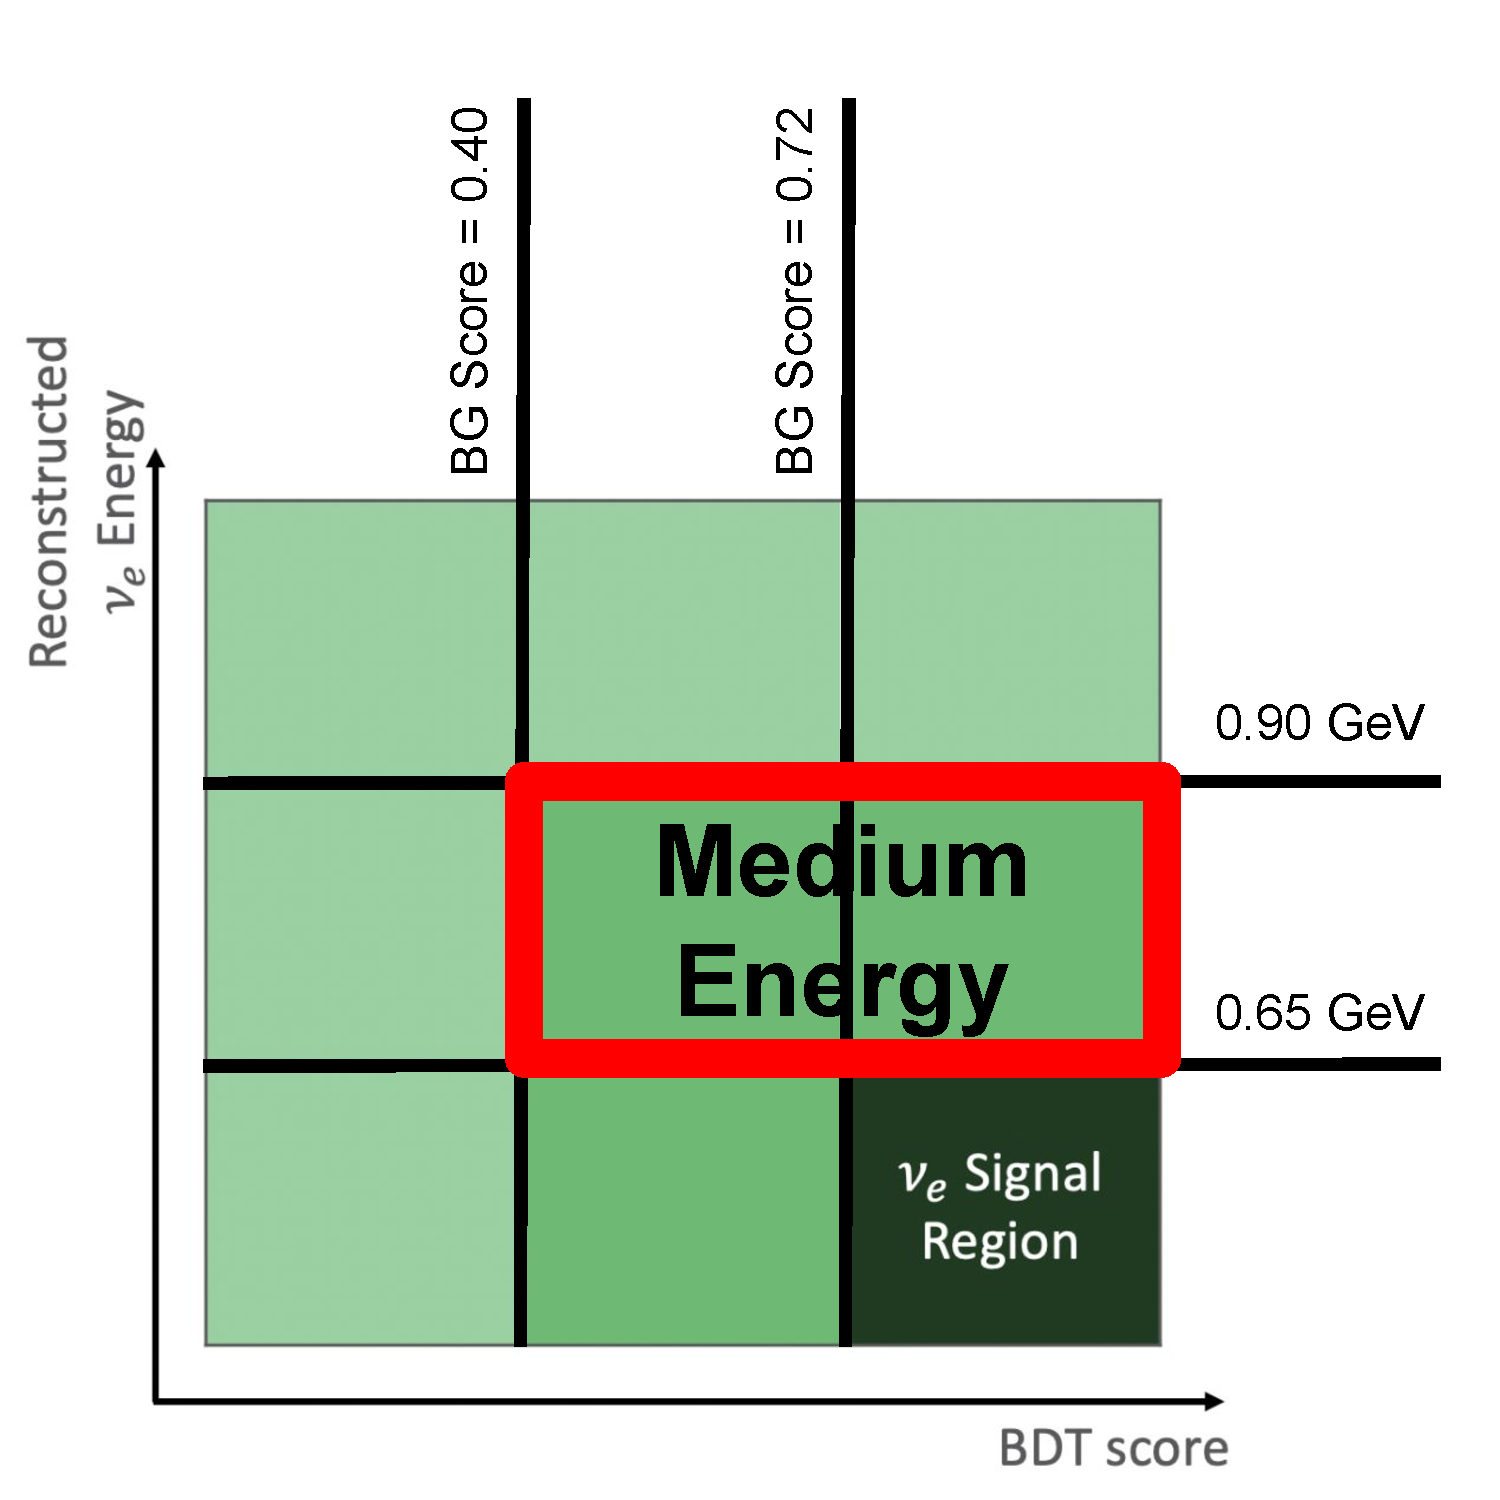
\includegraphics[width=\linewidth]{technote/Sidebands/Figures/NearSideband/ZpMediumEnergySideband.pdf}
        \caption{For the 1e0p selection.}
    \end{subfigure}%
    \begin{subfigure}{0.5\linewidth}
        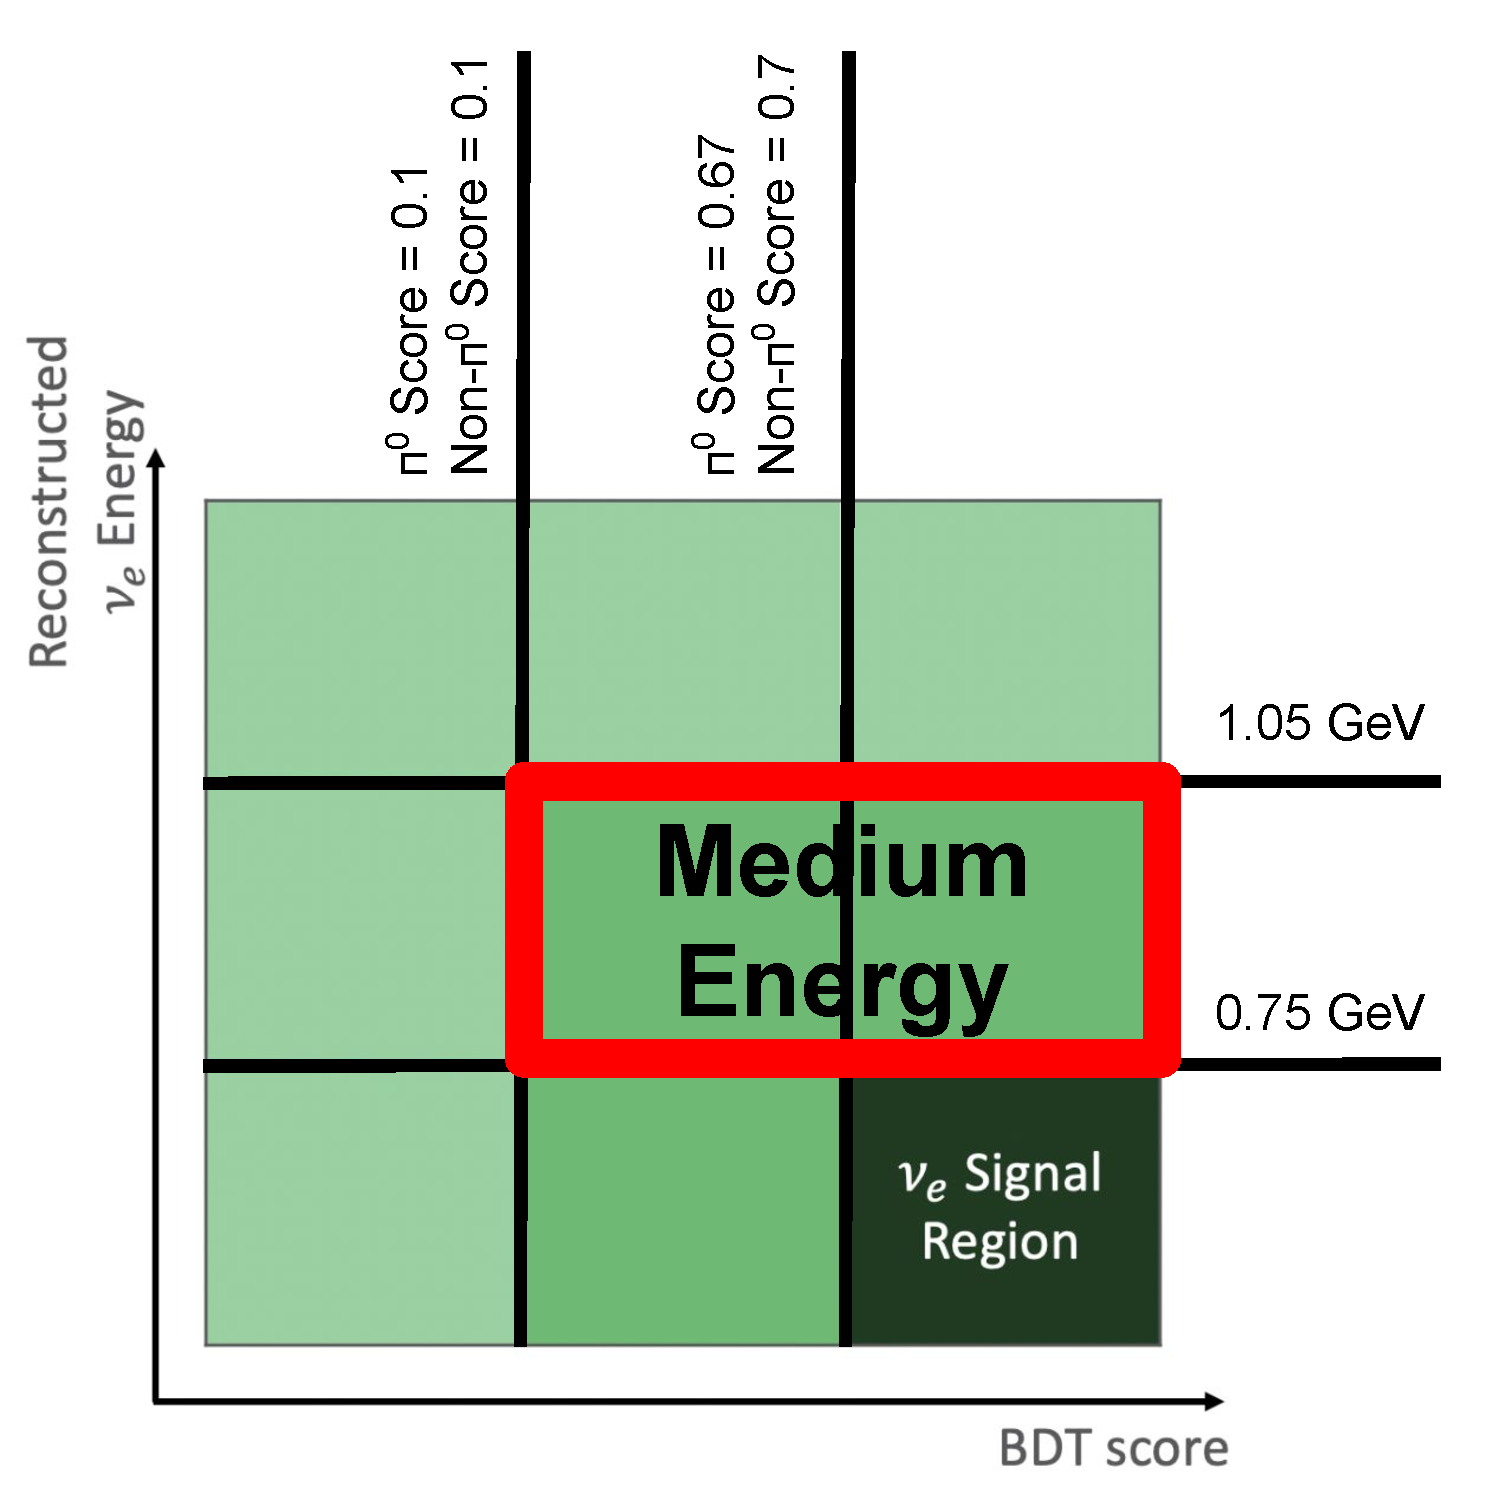
\includegraphics[width=\linewidth]{technote/Sidebands/Figures/NearSideband/NpMediumEnergySideband.pdf}
        \caption{For the 1eNp selection.}
    \end{subfigure}
    \caption{The medium energy sidebands.}
    \label{fig:MediumEnergySideband}
\end{figure}

\begin{figure}[H]
    \centering
    \begin{subfigure}{0.33\linewidth}
        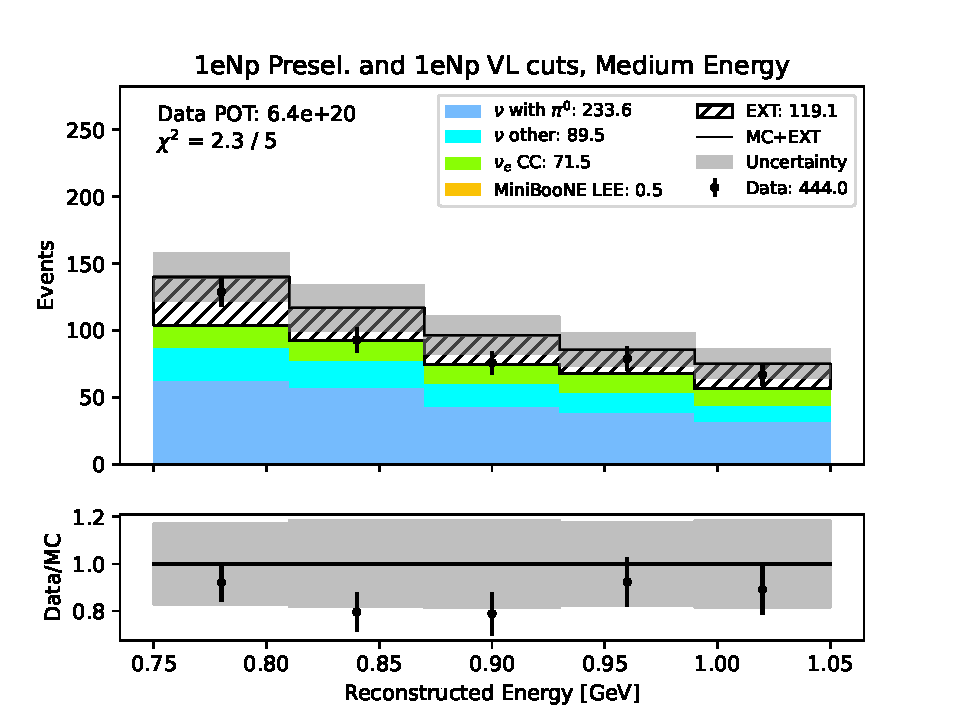
\includegraphics[width=\linewidth]{technote/Sidebands/Figures/NearSideband/near_sideband_reco_e_run123_NP_NP_MEDIUM_ENERGY.pdf}
        \caption{$\nu_e$ preselection, runs 1-3.}
    \end{subfigure}%
    \begin{subfigure}{0.33\linewidth}
        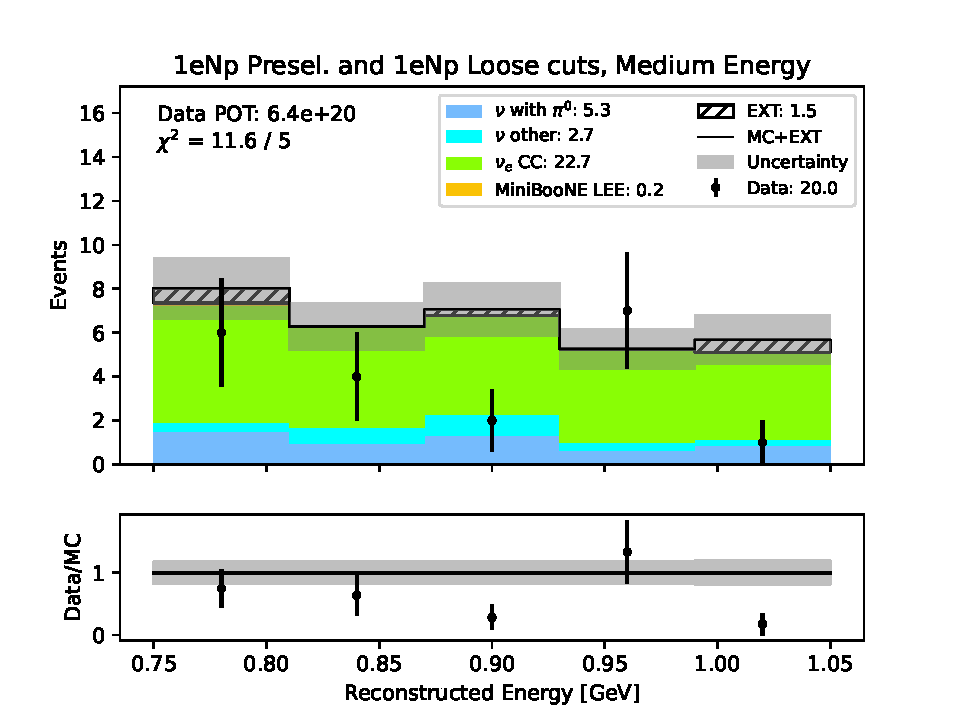
\includegraphics[width=\linewidth]{technote/Sidebands/Figures/NearSideband/near_sideband_reco_e_run123_NP_NPL_MEDIUM_ENERGY.pdf}
        \caption{1eNp loose selection, runs 1-3.}
    \end{subfigure}%
    \begin{subfigure}{0.33\linewidth}
        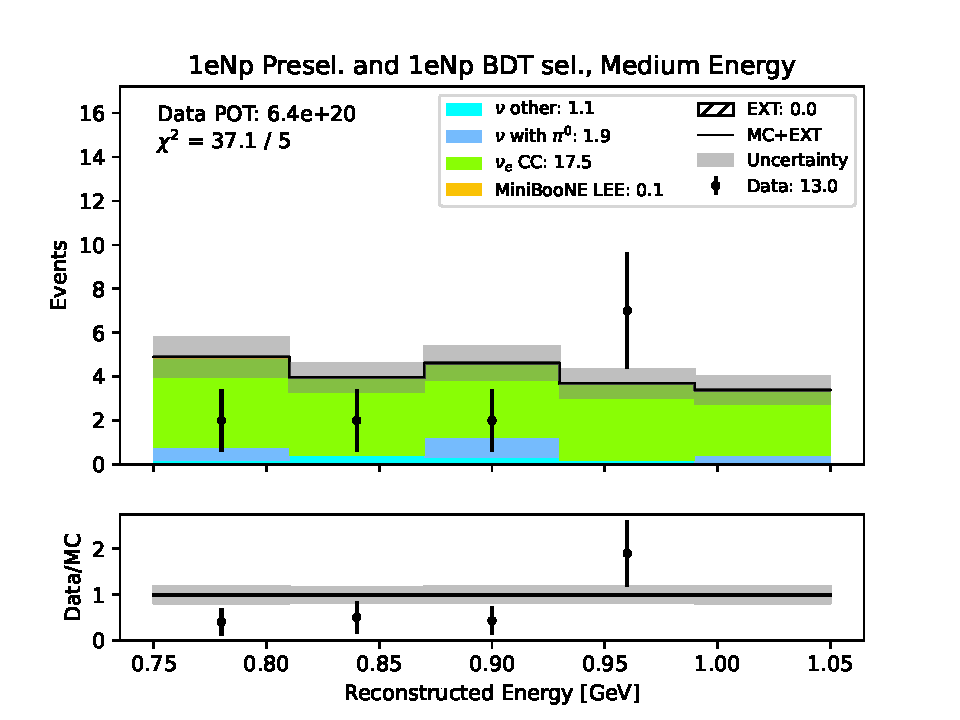
\includegraphics[width=\linewidth]{technote/Sidebands/Figures/NearSideband/near_sideband_reco_e_run123_NP_NPBDT_MEDIUM_ENERGY.pdf}
        \caption{1eNp BDT selection, runs 1-3.}
    \end{subfigure}
    \begin{subfigure}{0.33\linewidth}
        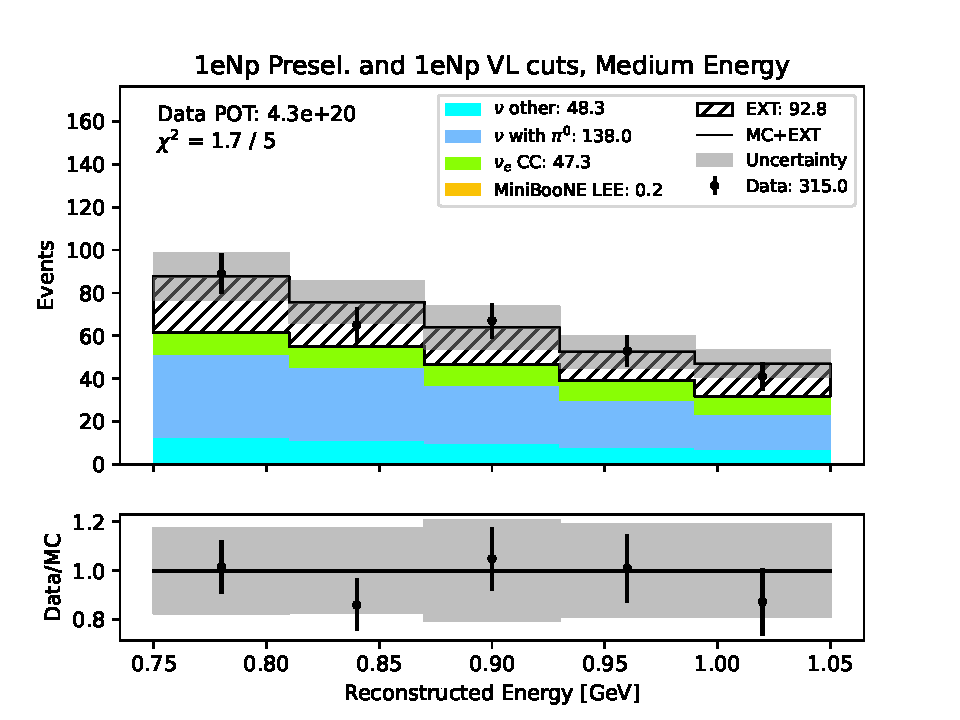
\includegraphics[width=\linewidth]{technote/Sidebands/Figures/NearSideband/near_sideband_reco_e_run4b4c4d5_NP_NP_MEDIUM_ENERGY.pdf}
        \caption{$\nu_e$ preselection, runs 4-5.}
    \end{subfigure}%
    \begin{subfigure}{0.33\linewidth}
        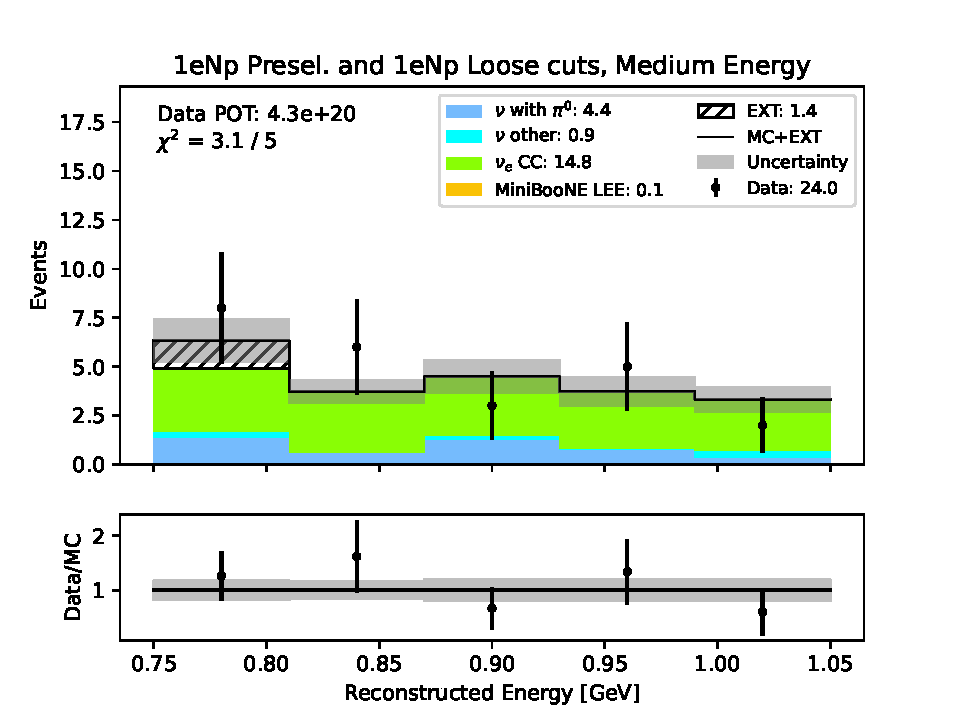
\includegraphics[width=\linewidth]{technote/Sidebands/Figures/NearSideband/near_sideband_reco_e_run4b4c4d5_NP_NPL_MEDIUM_ENERGY.pdf}
        \caption{1eNp loose selection, runs 4-5.}
    \end{subfigure}%
    \begin{subfigure}{0.33\linewidth}
        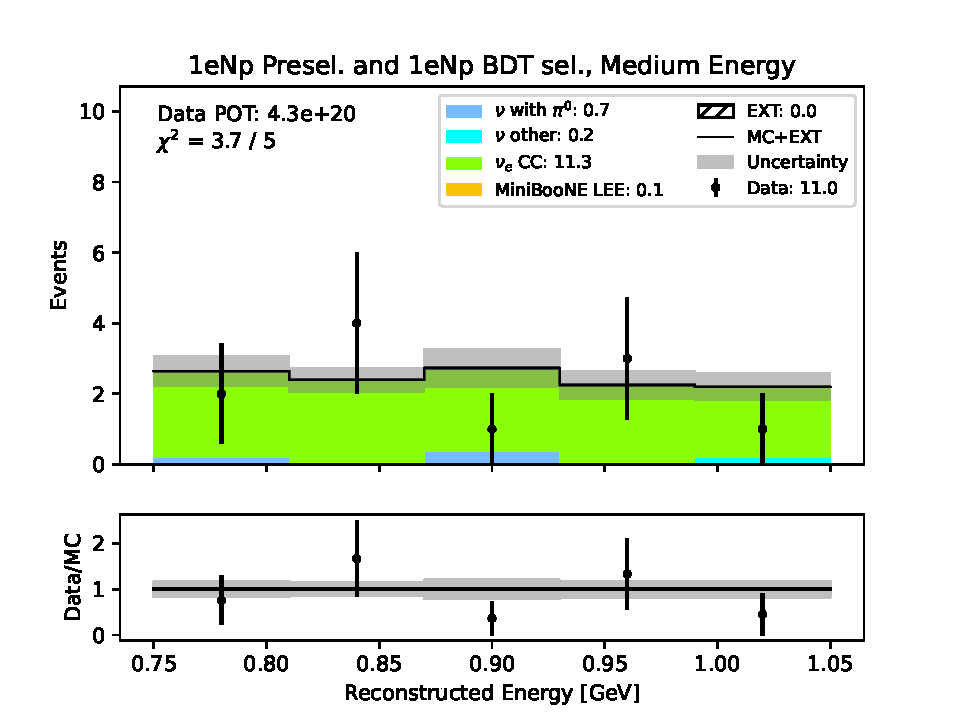
\includegraphics[width=\linewidth]{technote/Sidebands/Figures/NearSideband/near_sideband_reco_e_run4b4c4d5_NP_NPBDT_MEDIUM_ENERGY.pdf}
        \caption{1eNp BDT selection, runs 4-5.}
    \end{subfigure}
    \begin{subfigure}{0.33\linewidth}
        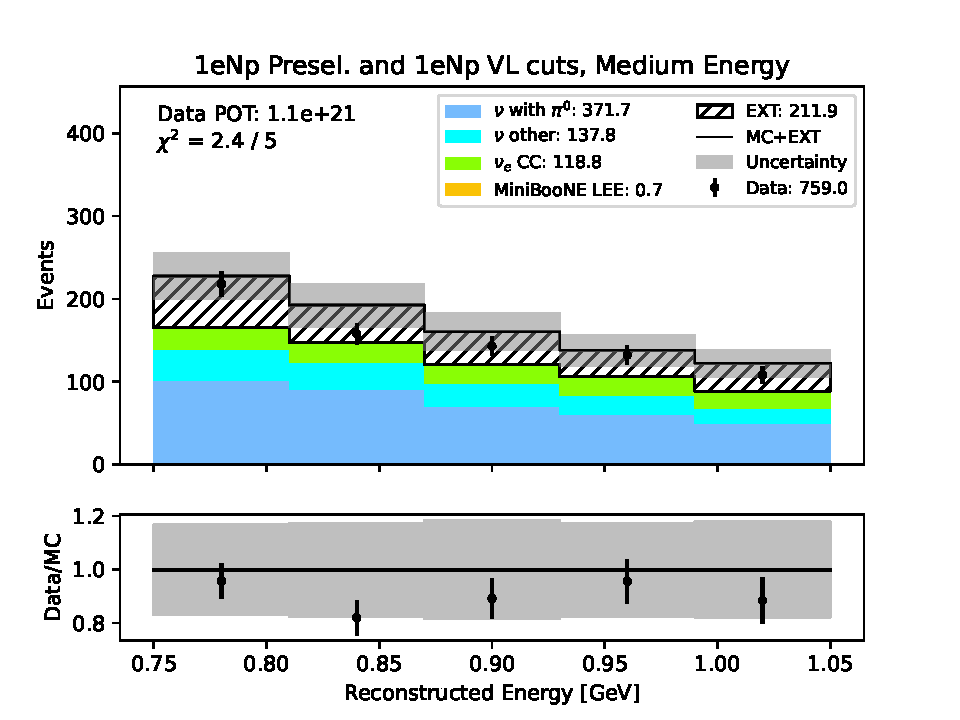
\includegraphics[width=\linewidth]{technote/Sidebands/Figures/NearSideband/near_sideband_reco_e_run1234b4c4d5_NP_NP_MEDIUM_ENERGY.pdf}
        \caption{$\nu_e$ preselection, runs 1-5.}
    \end{subfigure}%
    \begin{subfigure}{0.33\linewidth}
        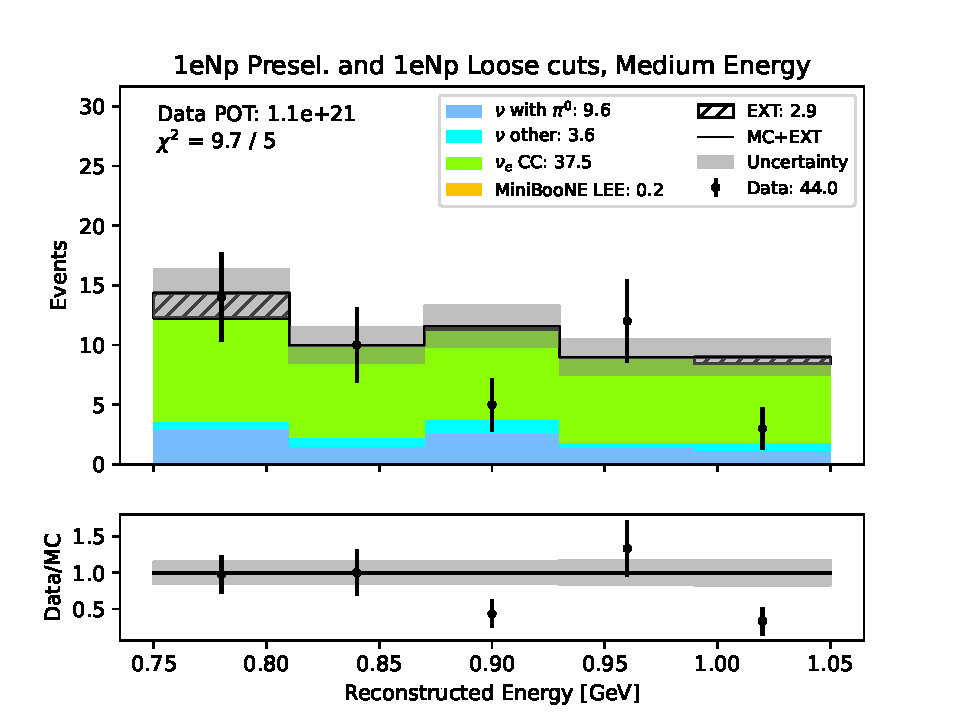
\includegraphics[width=\linewidth]{technote/Sidebands/Figures/NearSideband/near_sideband_reco_e_run1234b4c4d5_NP_NPL_MEDIUM_ENERGY.pdf}
        \caption{1eNp loose selection, runs 1-5.}
    \end{subfigure}%
    \begin{subfigure}{0.33\linewidth}
        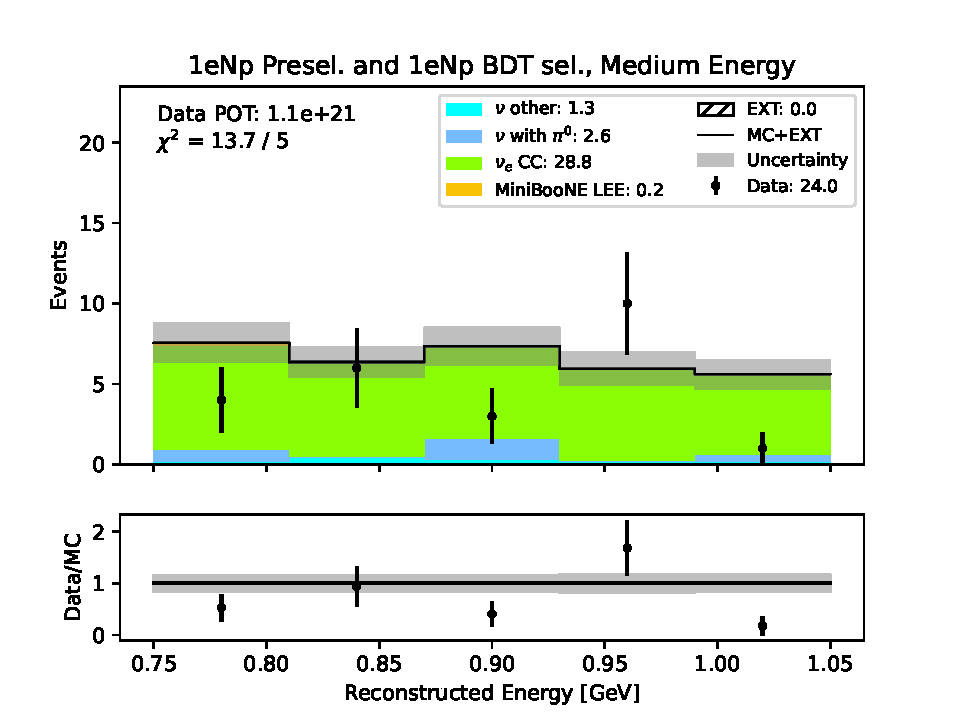
\includegraphics[width=\linewidth]{technote/Sidebands/Figures/NearSideband/near_sideband_reco_e_run1234b4c4d5_NP_NPBDT_MEDIUM_ENERGY.pdf}
        \caption{1eNp BDT selection, runs 1-5.}
    \end{subfigure}
    \caption{Data and MC simulation comparisons in the 1eNp medium energy sideband.}
\end{figure}

\begin{figure}[H]
    \centering
    \begin{subfigure}{0.33\linewidth}
        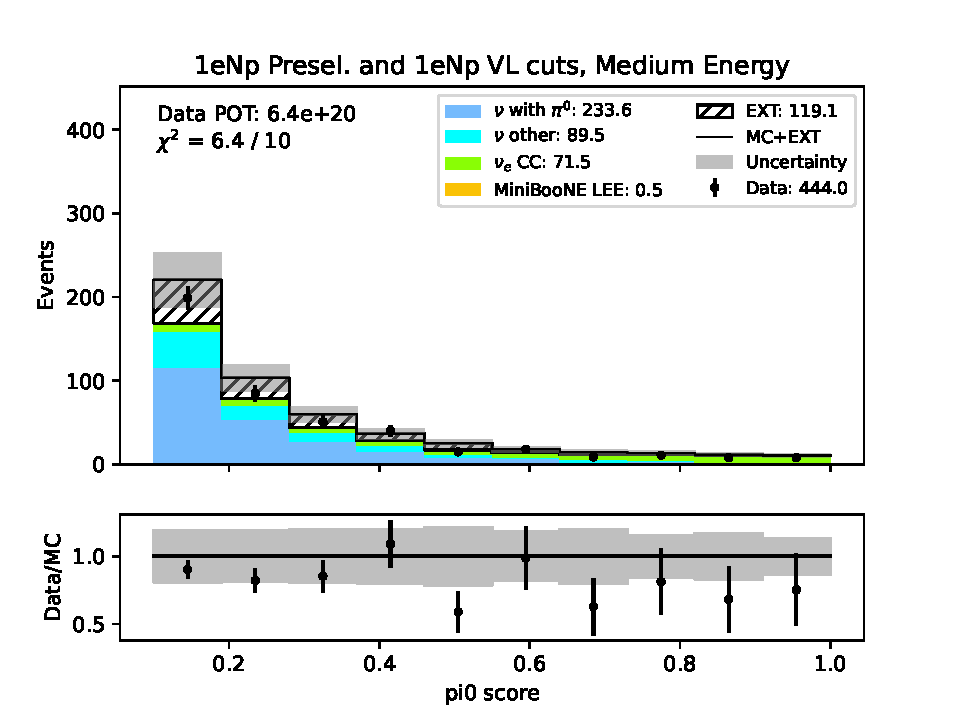
\includegraphics[width=\linewidth]{technote/Sidebands/Figures/NearSideband/near_sideband_pi0_score_run123_NP_NP_MEDIUM_ENERGY.pdf}
        \caption{$\nu_e$ preselection, runs 1-3.}
    \end{subfigure}%
    \begin{subfigure}{0.33\linewidth}
        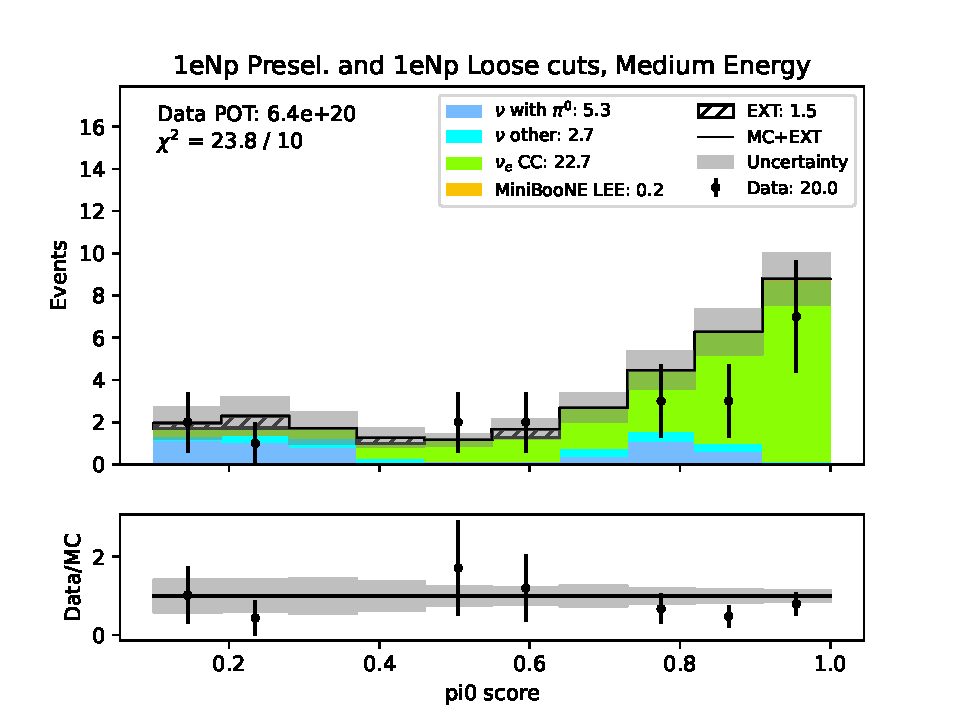
\includegraphics[width=\linewidth]{technote/Sidebands/Figures/NearSideband/near_sideband_pi0_score_run123_NP_NPL_MEDIUM_ENERGY.pdf}
        \caption{1eNp loose selection, runs 1-3.}
    \end{subfigure}%
    \begin{subfigure}{0.33\linewidth}
        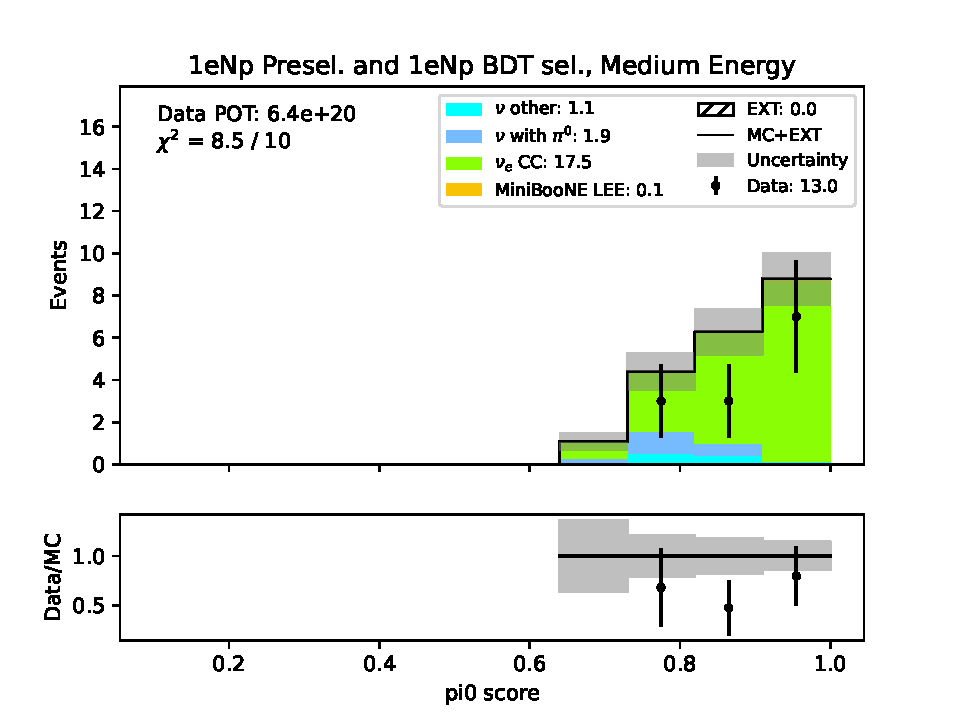
\includegraphics[width=\linewidth]{technote/Sidebands/Figures/NearSideband/near_sideband_pi0_score_run123_NP_NPBDT_MEDIUM_ENERGY.pdf}
        \caption{1eNp BDT selection, runs 1-3.}
    \end{subfigure}
    \begin{subfigure}{0.33\linewidth}
        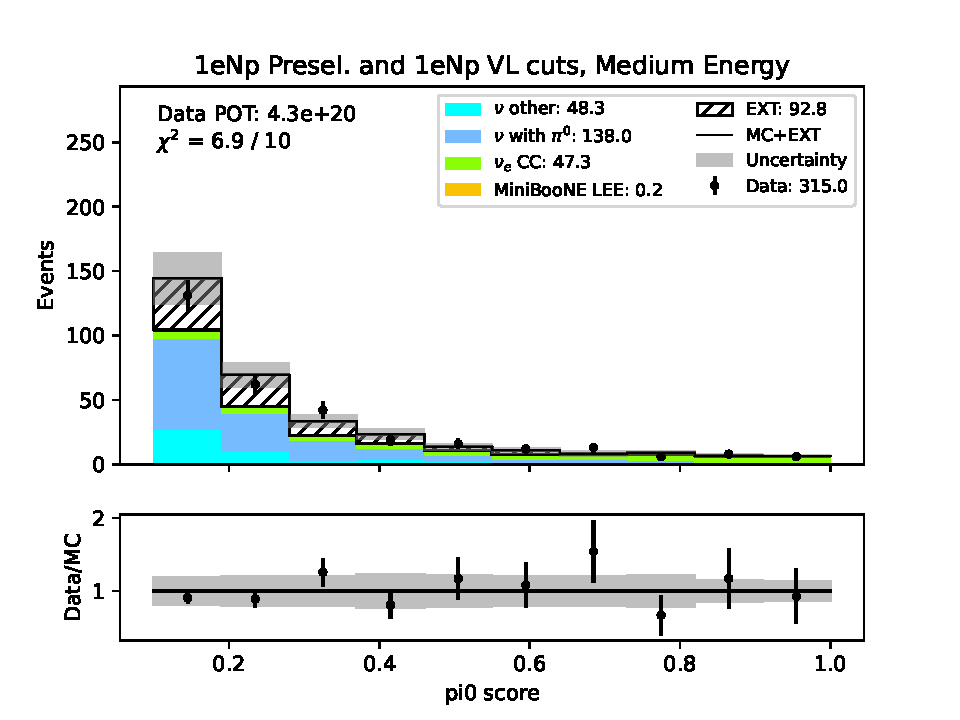
\includegraphics[width=\linewidth]{technote/Sidebands/Figures/NearSideband/near_sideband_pi0_score_run4b4c4d5_NP_NP_MEDIUM_ENERGY.pdf}
        \caption{$\nu_e$ preselection, runs 4-5.}
    \end{subfigure}%
    \begin{subfigure}{0.33\linewidth}
        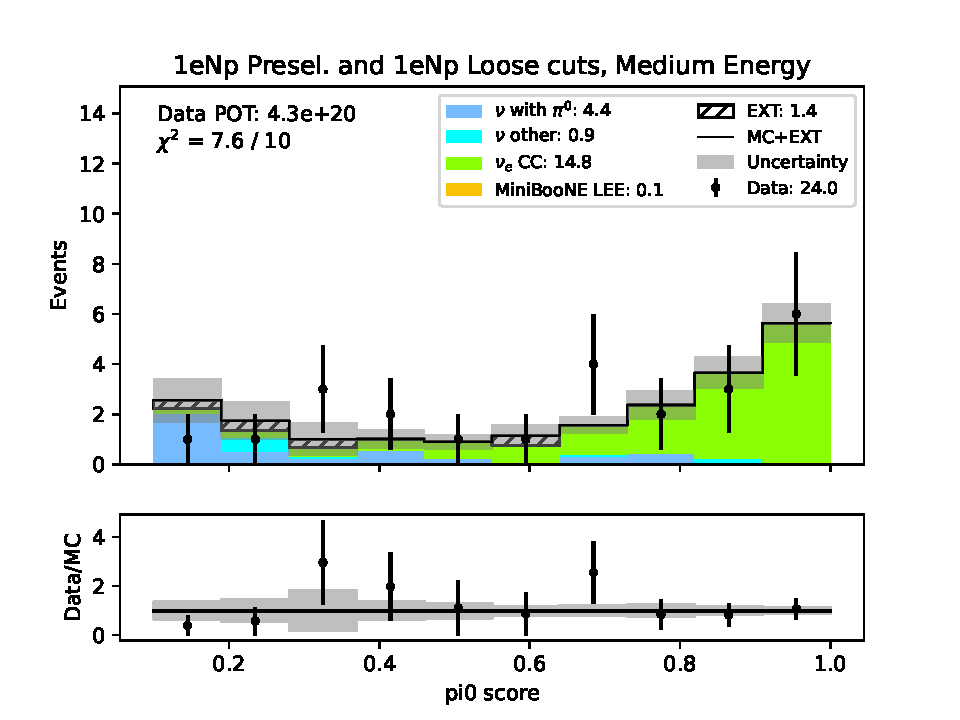
\includegraphics[width=\linewidth]{technote/Sidebands/Figures/NearSideband/near_sideband_pi0_score_run4b4c4d5_NP_NPL_MEDIUM_ENERGY.pdf}
        \caption{1eNp loose selection, runs 4-5.}
    \end{subfigure}%
    \begin{subfigure}{0.33\linewidth}
        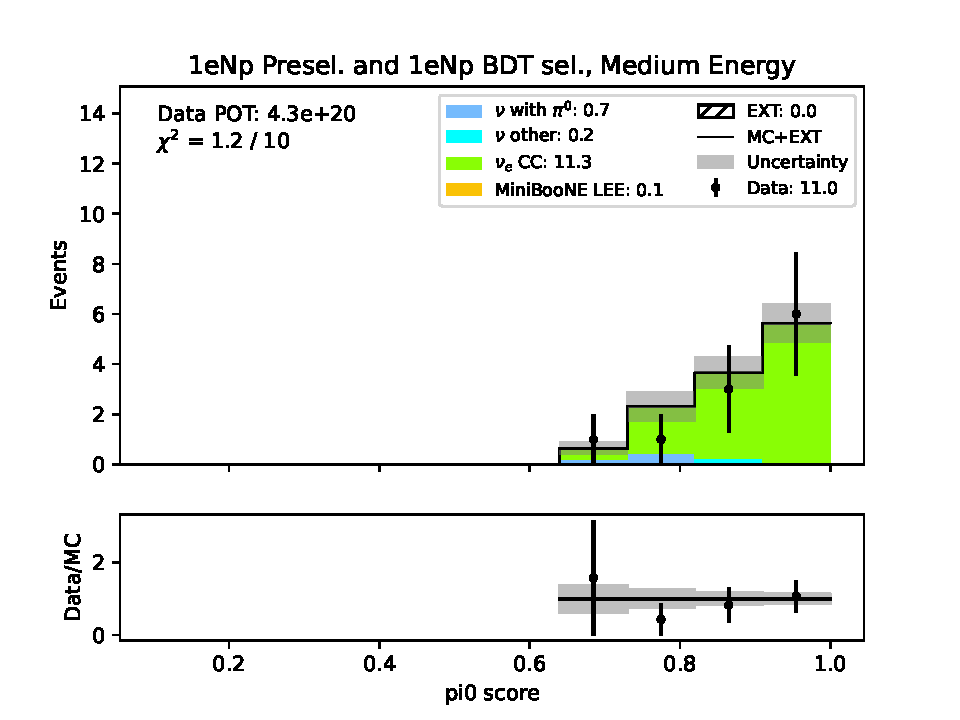
\includegraphics[width=\linewidth]{technote/Sidebands/Figures/NearSideband/near_sideband_pi0_score_run4b4c4d5_NP_NPBDT_MEDIUM_ENERGY.pdf}
        \caption{1eNp BDT selection, runs 4-5.}
    \end{subfigure}
    \begin{subfigure}{0.33\linewidth}
        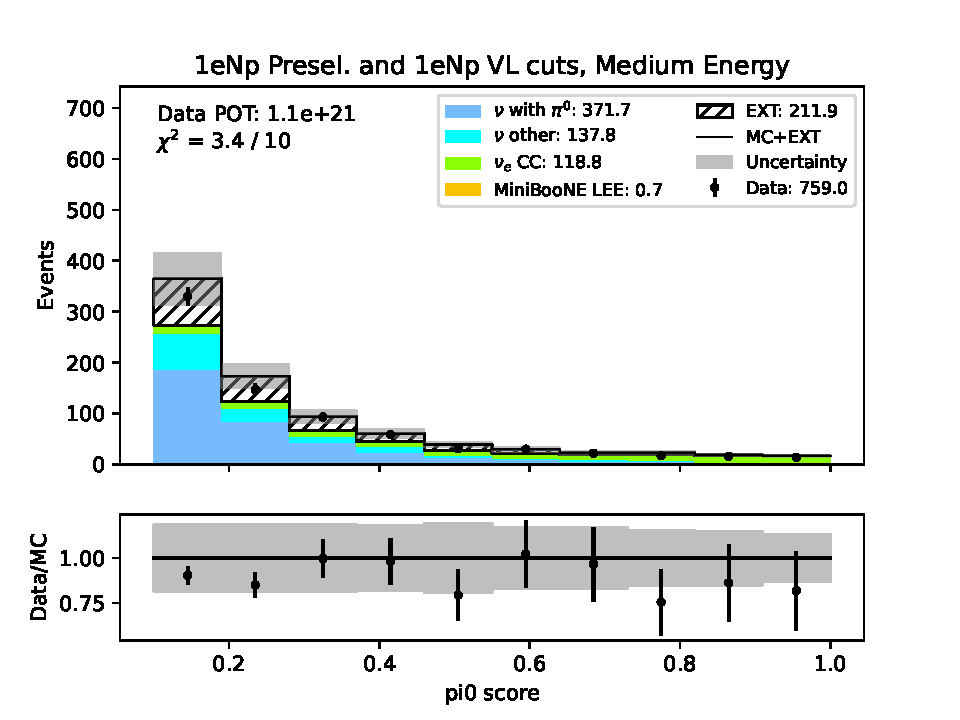
\includegraphics[width=\linewidth]{technote/Sidebands/Figures/NearSideband/near_sideband_pi0_score_run1234b4c4d5_NP_NP_MEDIUM_ENERGY.pdf}
        \caption{$\nu_e$ preselection, runs 1-5.}
    \end{subfigure}%
    \begin{subfigure}{0.33\linewidth}
        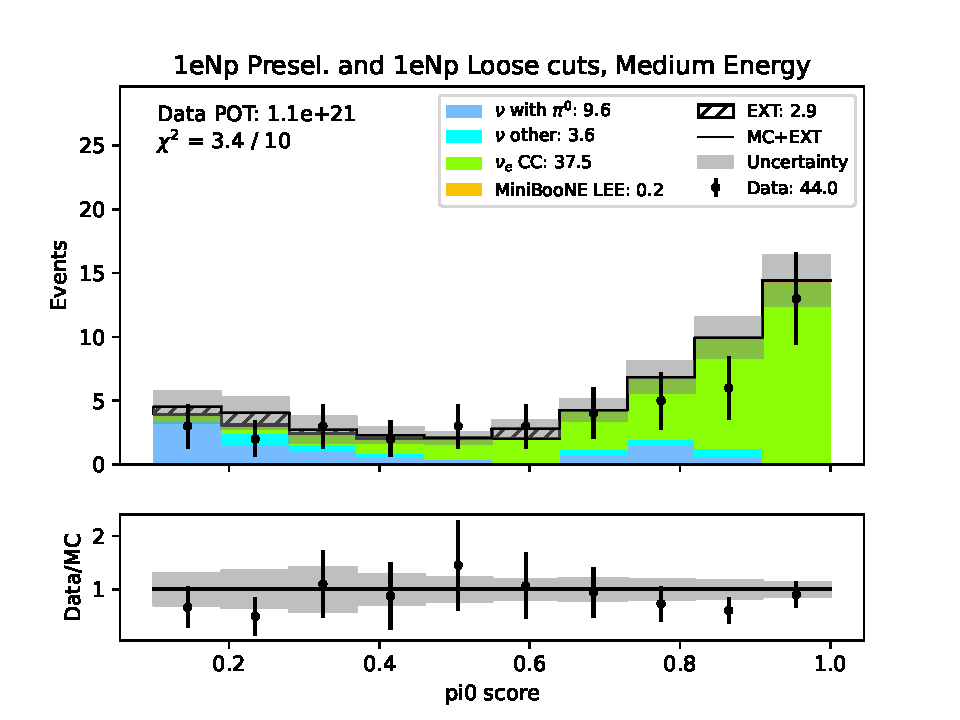
\includegraphics[width=\linewidth]{technote/Sidebands/Figures/NearSideband/near_sideband_pi0_score_run1234b4c4d5_NP_NPL_MEDIUM_ENERGY.pdf}
        \caption{1eNp loose selection, runs 1-5.}
    \end{subfigure}%
    \begin{subfigure}{0.33\linewidth}
        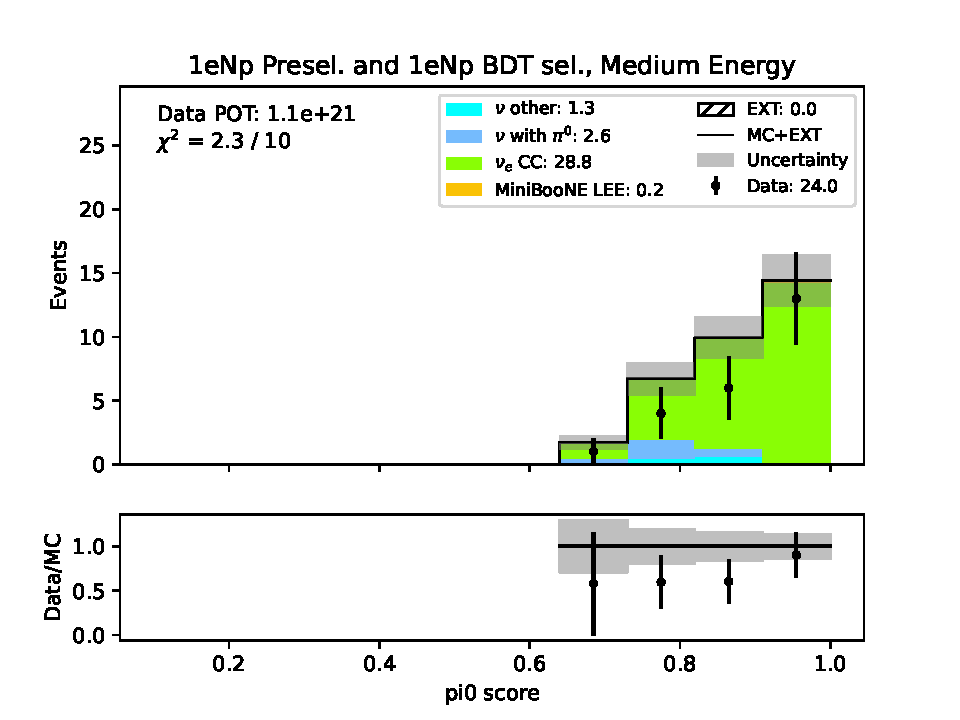
\includegraphics[width=\linewidth]{technote/Sidebands/Figures/NearSideband/near_sideband_pi0_score_run1234b4c4d5_NP_NPBDT_MEDIUM_ENERGY.pdf}
        \caption{1eNp BDT selection, runs 1-5.}
    \end{subfigure}
    \caption{Data and MC simulation comparisons in the 1eNp medium energy sideband.}
\end{figure}

\begin{figure}[H]
    \centering
    \begin{subfigure}{0.33\linewidth}
        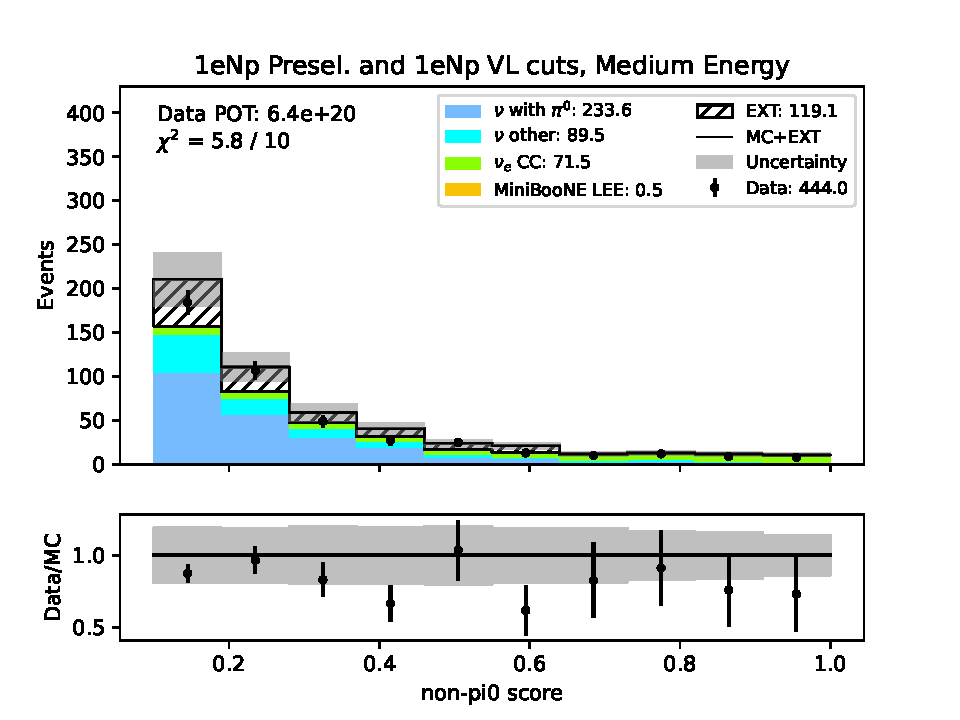
\includegraphics[width=\linewidth]{technote/Sidebands/Figures/NearSideband/near_sideband_nonpi0_score_run123_NP_NP_MEDIUM_ENERGY.pdf}
        \caption{$\nu_e$ preselection, runs 1-3.}
    \end{subfigure}%
    \begin{subfigure}{0.33\linewidth}
        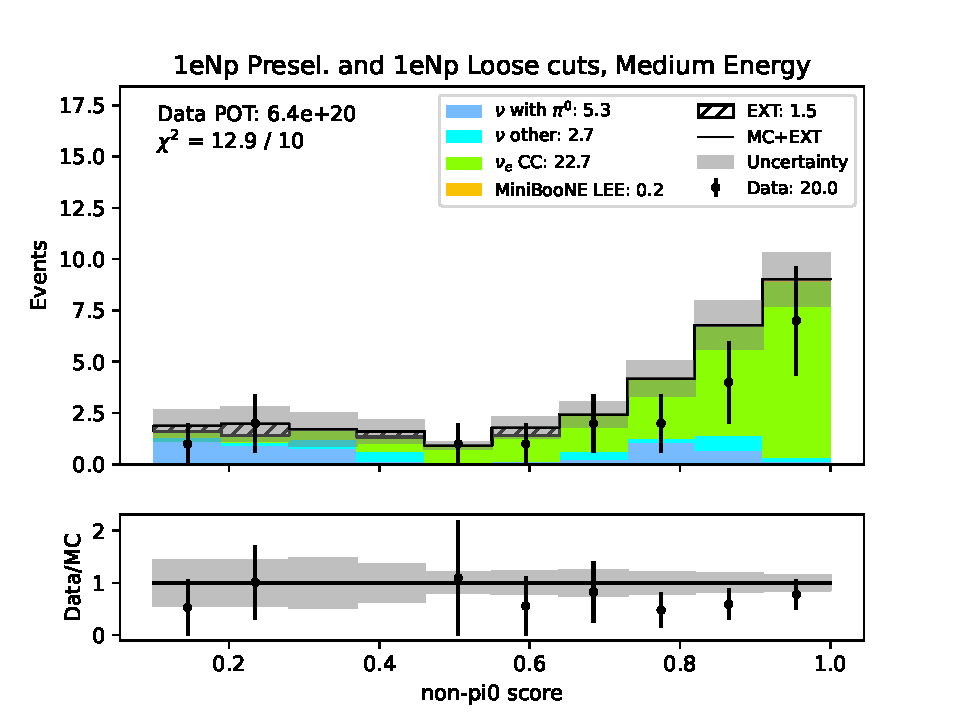
\includegraphics[width=\linewidth]{technote/Sidebands/Figures/NearSideband/near_sideband_nonpi0_score_run123_NP_NPL_MEDIUM_ENERGY.pdf}
        \caption{1eNp loose selection, runs 1-3.}
    \end{subfigure}%
    \begin{subfigure}{0.33\linewidth}
        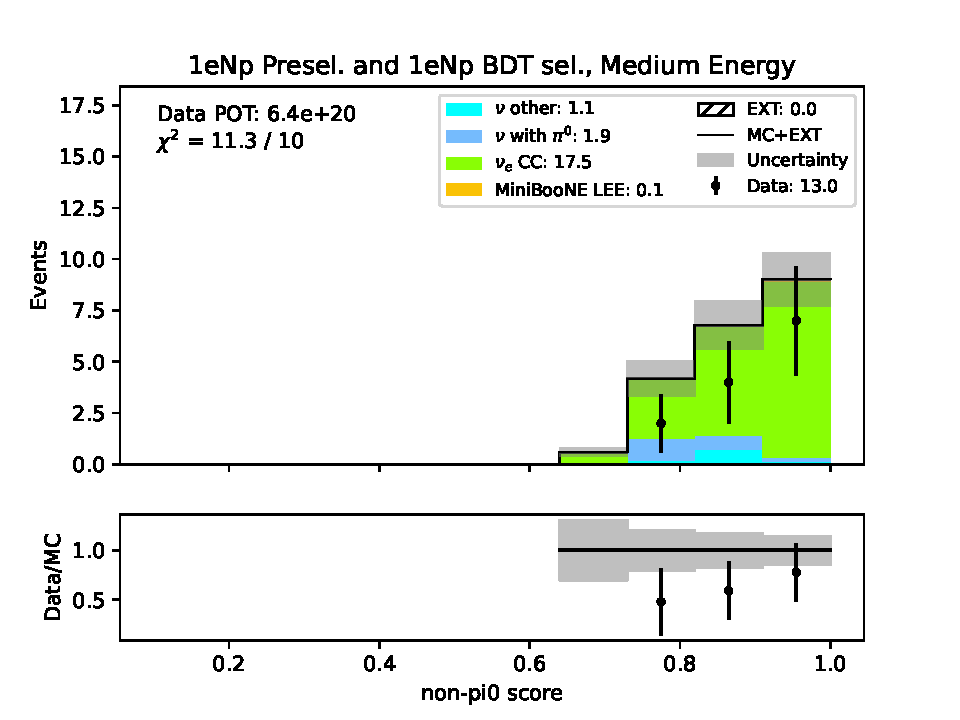
\includegraphics[width=\linewidth]{technote/Sidebands/Figures/NearSideband/near_sideband_nonpi0_score_run123_NP_NPBDT_MEDIUM_ENERGY.pdf}
        \caption{1eNp BDT selection, runs 1-3.}
    \end{subfigure}
    \begin{subfigure}{0.33\linewidth}
        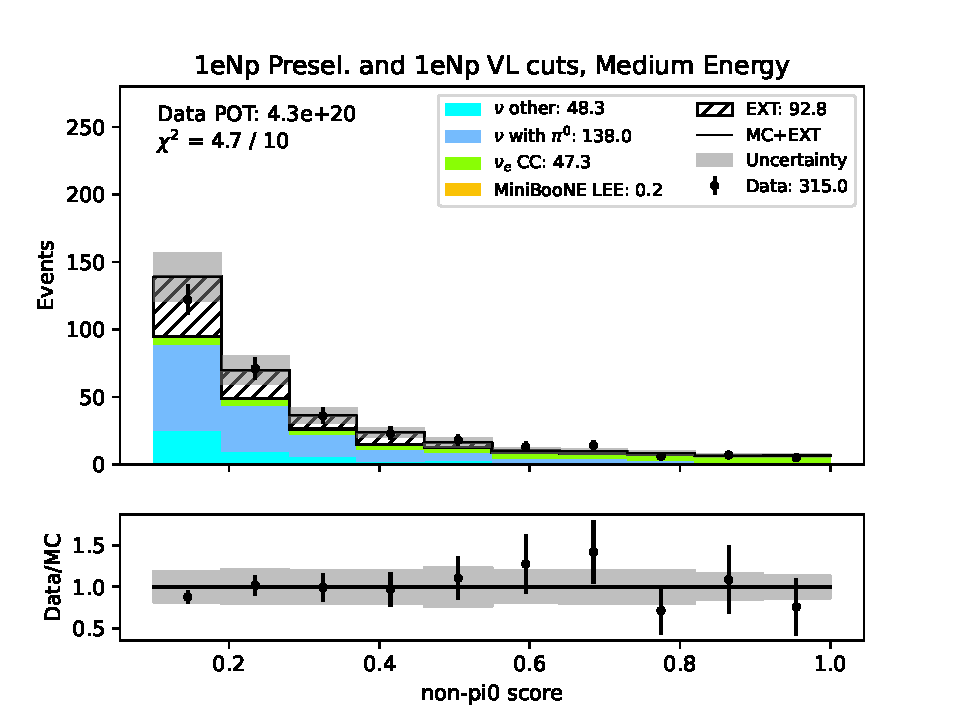
\includegraphics[width=\linewidth]{technote/Sidebands/Figures/NearSideband/near_sideband_nonpi0_score_run4b4c4d5_NP_NP_MEDIUM_ENERGY.pdf}
        \caption{$\nu_e$ preselection, runs 4-5.}
    \end{subfigure}%
    \begin{subfigure}{0.33\linewidth}
        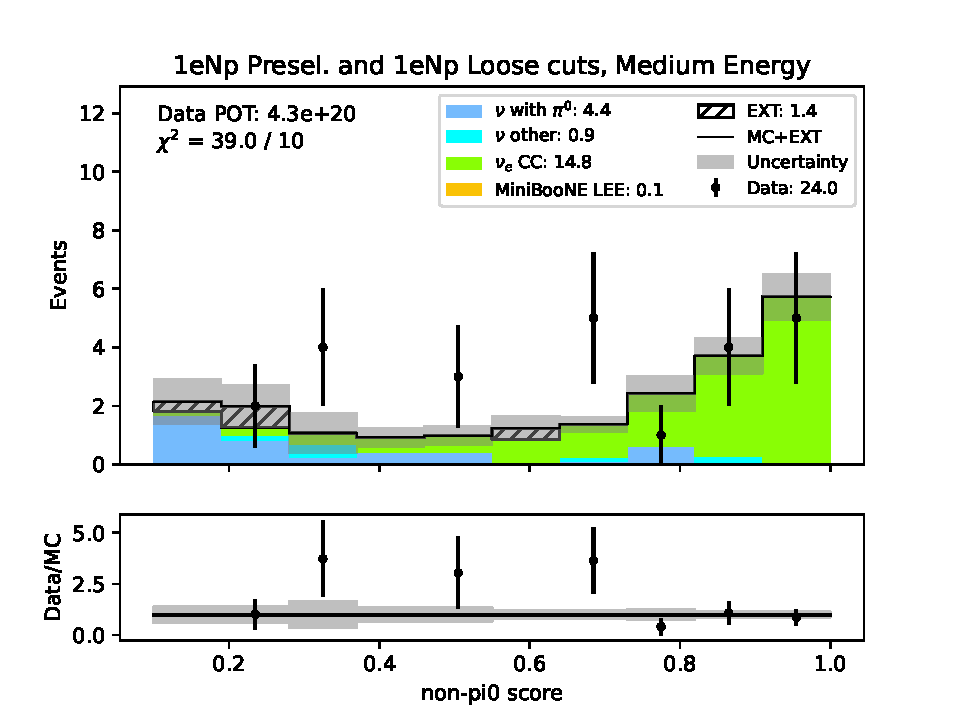
\includegraphics[width=\linewidth]{technote/Sidebands/Figures/NearSideband/near_sideband_nonpi0_score_run4b4c4d5_NP_NPL_MEDIUM_ENERGY.pdf}
        \caption{1eNp loose selection, runs 4-5.}
    \end{subfigure}%
    \begin{subfigure}{0.33\linewidth}
        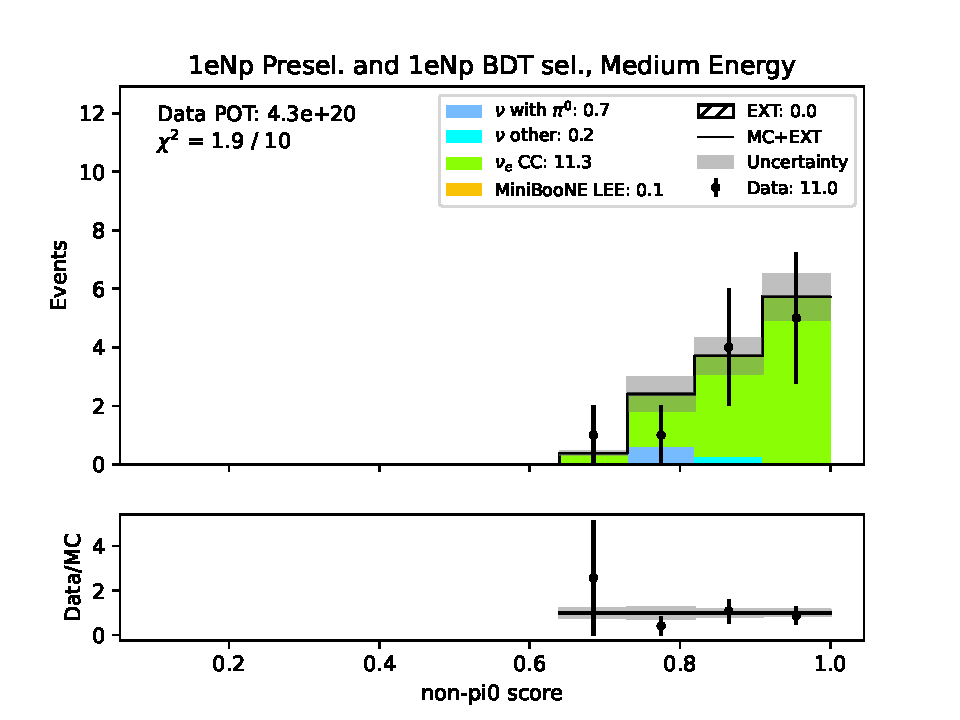
\includegraphics[width=\linewidth]{technote/Sidebands/Figures/NearSideband/near_sideband_nonpi0_score_run4b4c4d5_NP_NPBDT_MEDIUM_ENERGY.pdf}
        \caption{1eNp BDT selection, runs 4-5.}
    \end{subfigure}    
    \begin{subfigure}{0.33\linewidth}
        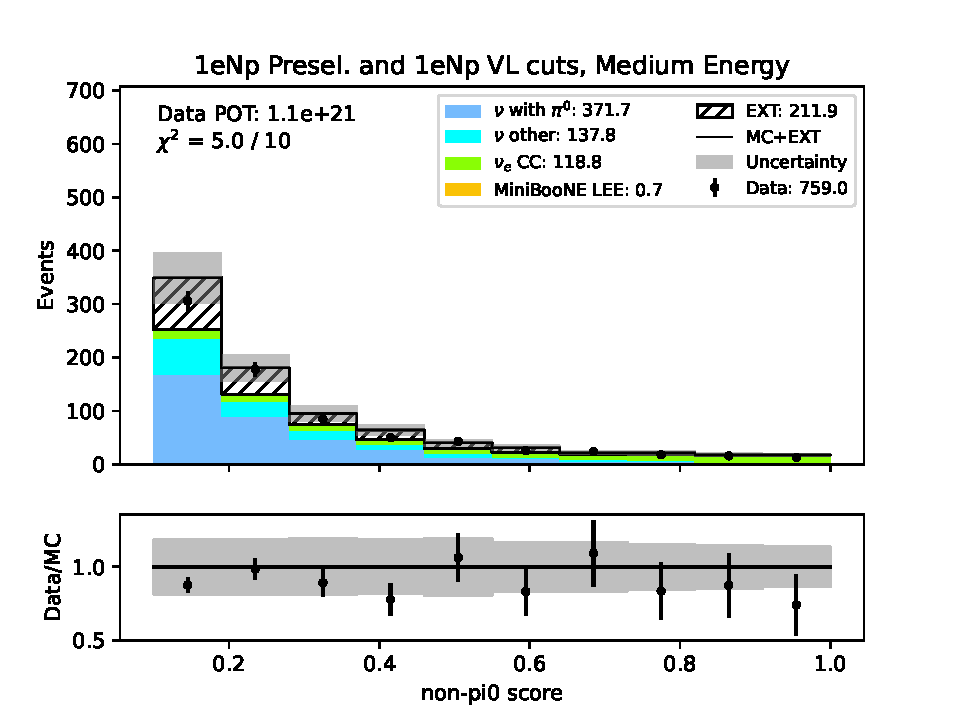
\includegraphics[width=\linewidth]{technote/Sidebands/Figures/NearSideband/near_sideband_nonpi0_score_run1234b4c4d5_NP_NP_MEDIUM_ENERGY.pdf}
        \caption{$\nu_e$ preselection, runs 1-5.}
    \end{subfigure}%
    \begin{subfigure}{0.33\linewidth}
        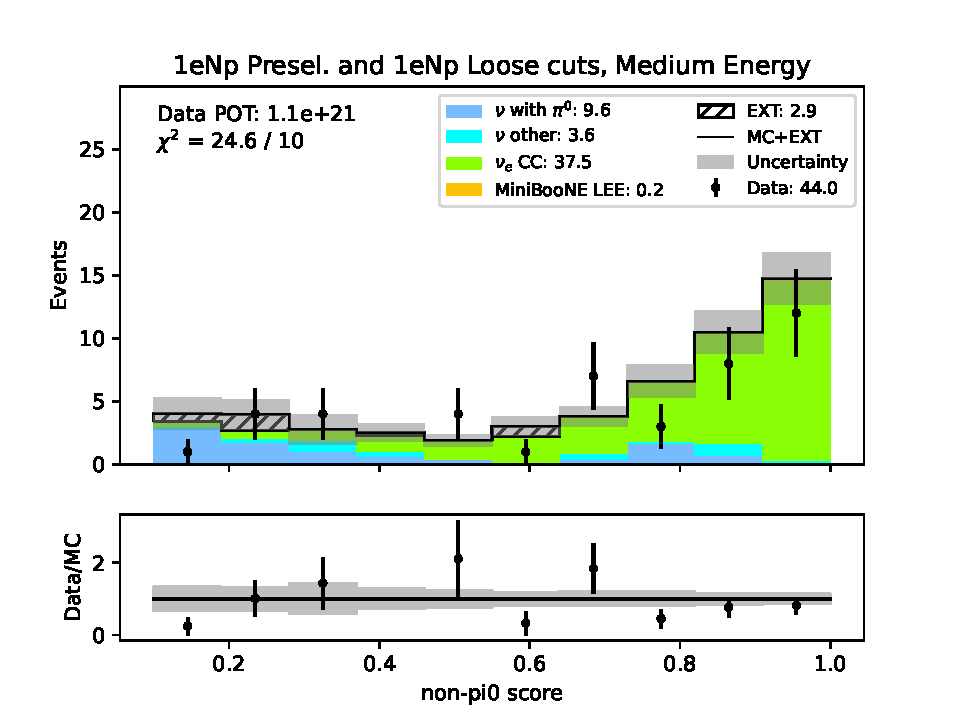
\includegraphics[width=\linewidth]{technote/Sidebands/Figures/NearSideband/near_sideband_nonpi0_score_run1234b4c4d5_NP_NPL_MEDIUM_ENERGY.pdf}
        \caption{1eNp loose selection, runs 1-5.}
    \end{subfigure}%
    \begin{subfigure}{0.33\linewidth}
        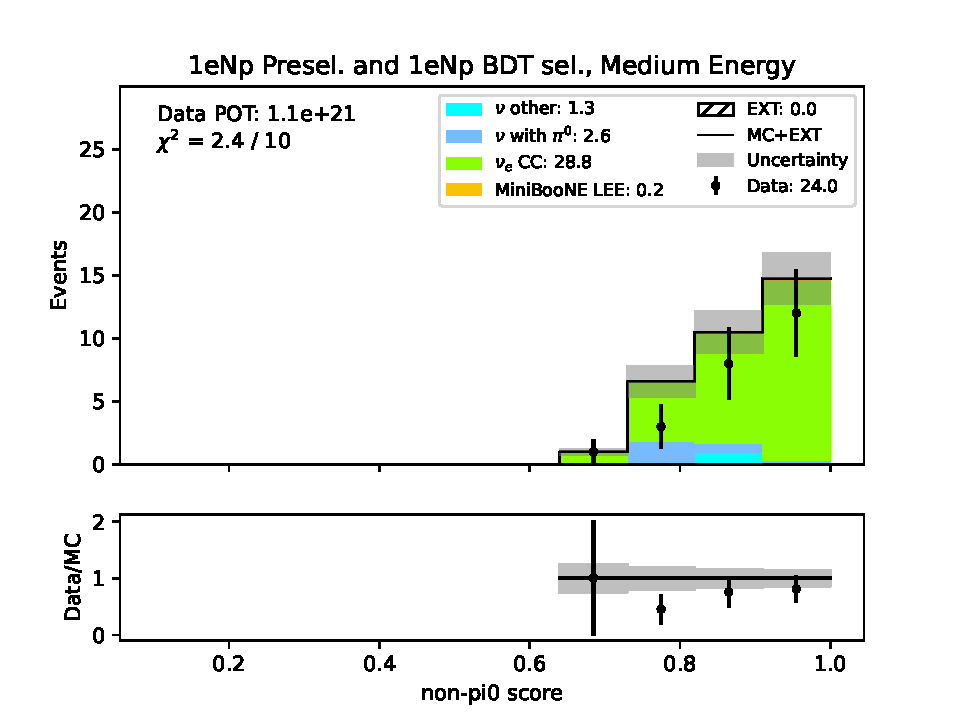
\includegraphics[width=\linewidth]{technote/Sidebands/Figures/NearSideband/near_sideband_nonpi0_score_run1234b4c4d5_NP_NPBDT_MEDIUM_ENERGY.pdf}
        \caption{1eNp BDT selection, runs 1-5.}
    \end{subfigure}
    \caption{Data and MC simulation comparisons in the 1eNp medium energy sideband.}
\end{figure}

\begin{figure}[H]
    \centering
    \begin{subfigure}{0.5\linewidth}
        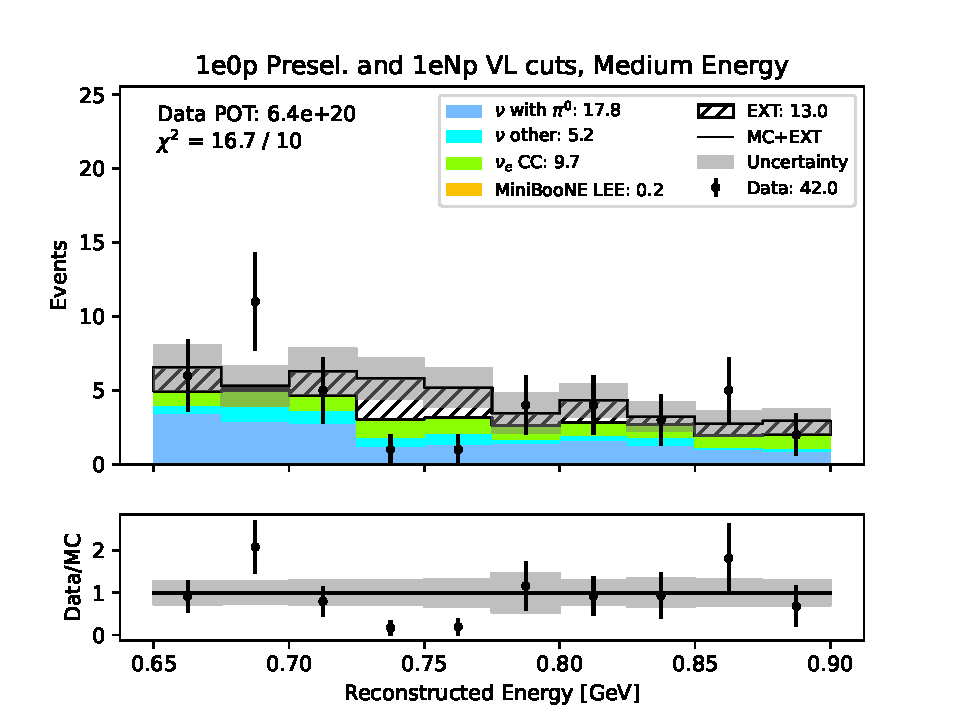
\includegraphics[width=\linewidth]{technote/Sidebands/Figures/NearSideband/near_sideband_reco_e_run123_ZP_ZP_MEDIUM_ENERGY.pdf}
        \caption{$\nu_e$ preselection, runs 1-3.}
    \end{subfigure}%
    \begin{subfigure}{0.5\linewidth}
        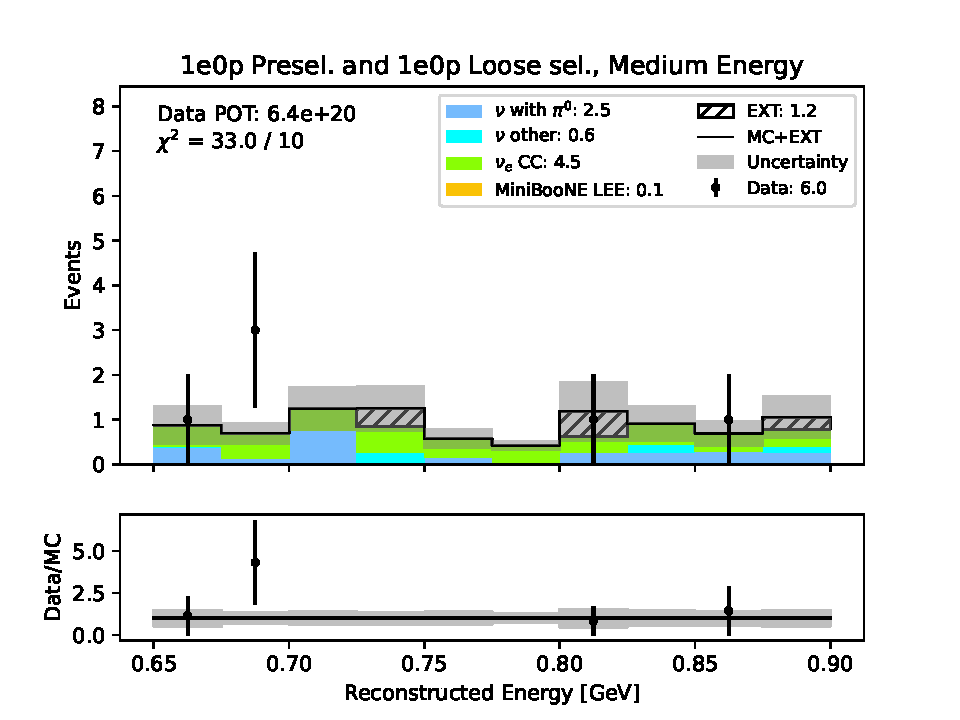
\includegraphics[width=\linewidth]{technote/Sidebands/Figures/NearSideband/near_sideband_reco_e_run123_ZP_ZPLOOSESEL_MEDIUM_ENERGY.pdf}
        \caption{Loose selection, runs 1-3.}
    \end{subfigure}
    \begin{subfigure}{0.5\linewidth}
        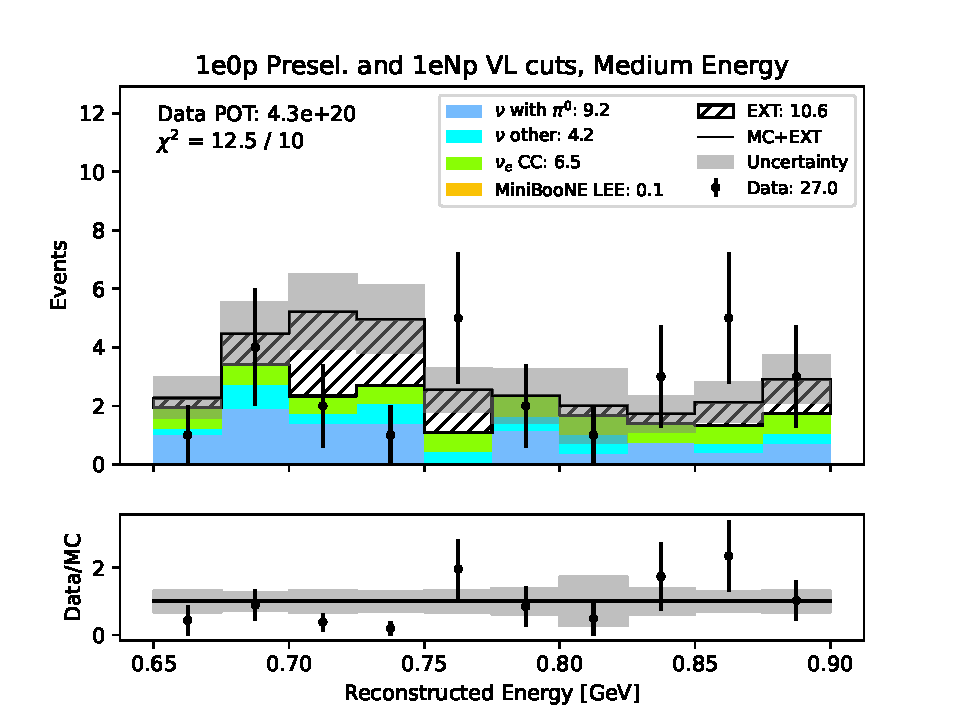
\includegraphics[width=\linewidth]{technote/Sidebands/Figures/NearSideband/near_sideband_reco_e_run4b4c4d5_ZP_ZP_MEDIUM_ENERGY.pdf}
        \caption{$\nu_e$ preselection, runs 4-5.}
    \end{subfigure}%
    \begin{subfigure}{0.5\linewidth}
        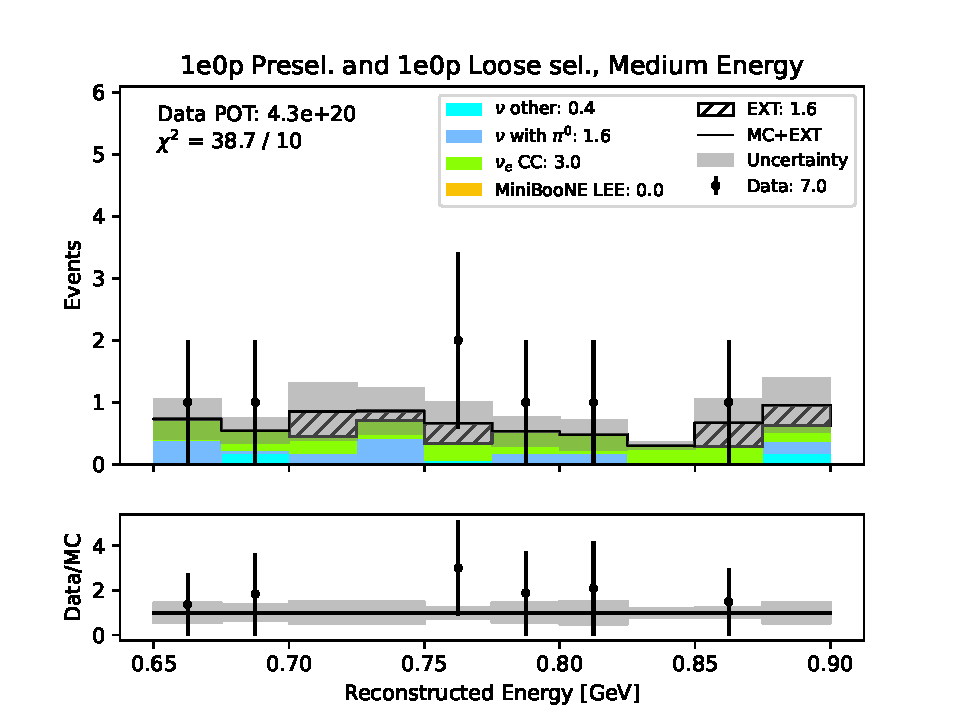
\includegraphics[width=\linewidth]{technote/Sidebands/Figures/NearSideband/near_sideband_reco_e_run4b4c4d5_ZP_ZPLOOSESEL_MEDIUM_ENERGY.pdf}
        \caption{Loose selection, runs 4-5.}
    \end{subfigure}
    \begin{subfigure}{0.5\linewidth}
        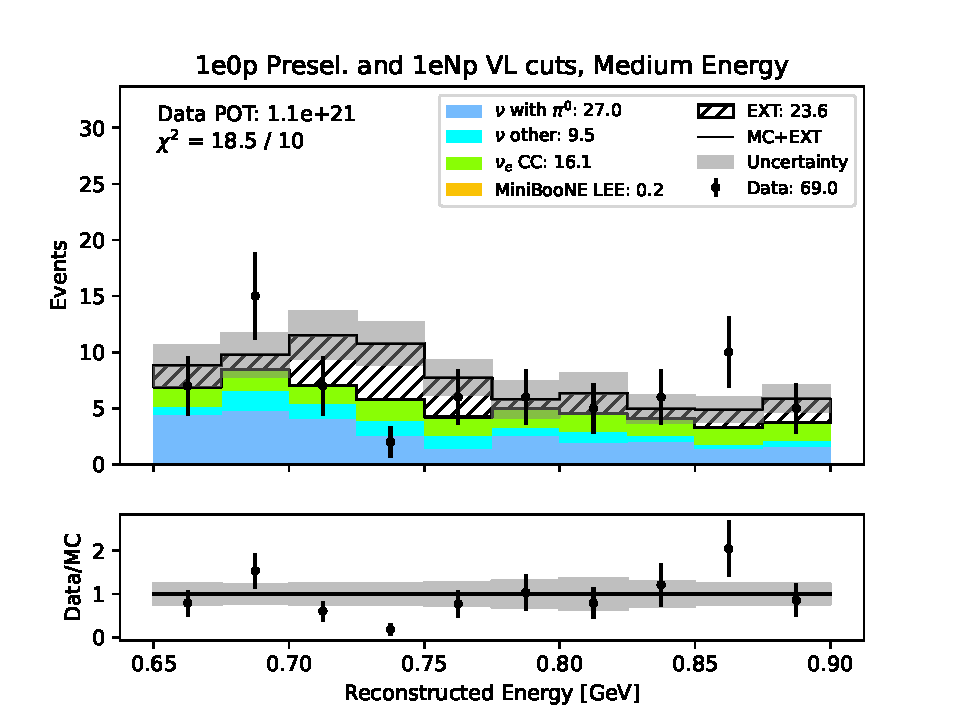
\includegraphics[width=\linewidth]{technote/Sidebands/Figures/NearSideband/near_sideband_reco_e_run1234b4c4d5_ZP_ZP_MEDIUM_ENERGY.pdf}
        \caption{$\nu_e$ preselection, runs 1-5.}
    \end{subfigure}%
    \begin{subfigure}{0.5\linewidth}
        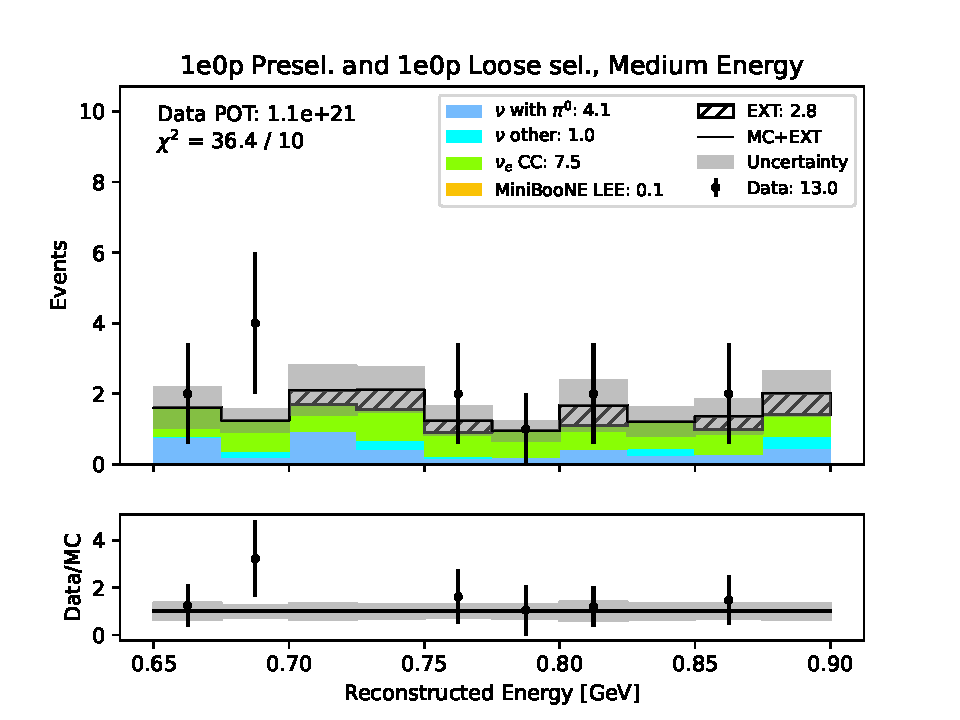
\includegraphics[width=\linewidth]{technote/Sidebands/Figures/NearSideband/near_sideband_reco_e_run1234b4c4d5_ZP_ZPLOOSESEL_MEDIUM_ENERGY.pdf}
        \caption{Loose selection, runs 1-5.}
    \end{subfigure}
    \caption{Data and MC simulation comparisons in the 1e0p medium energy sideband.}
\end{figure}

\begin{figure}[H]
    \centering
    \begin{subfigure}{0.5\linewidth}
        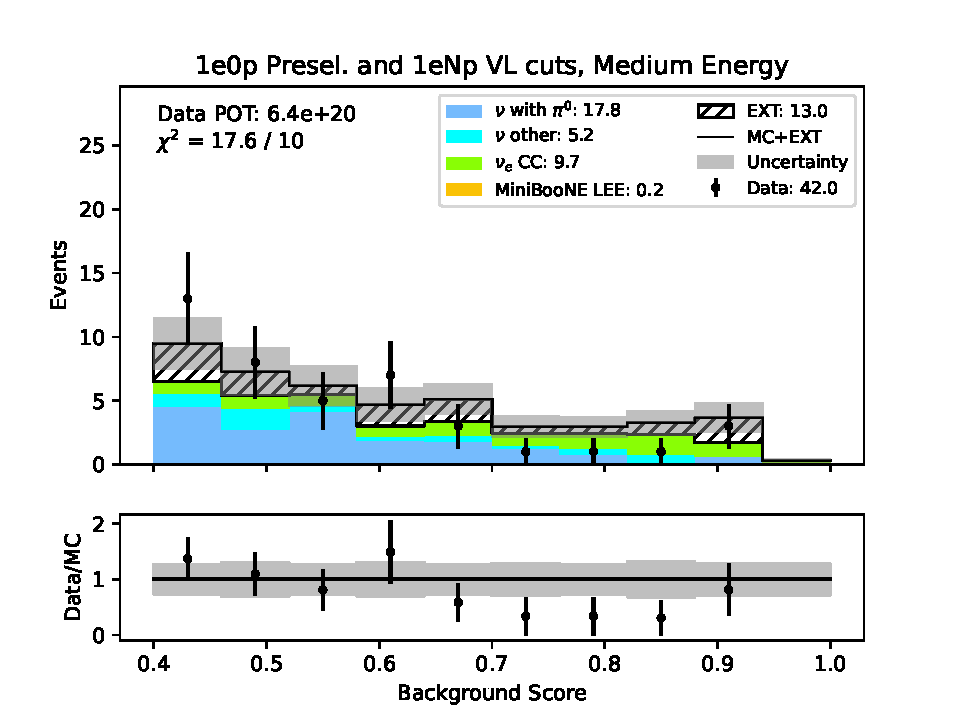
\includegraphics[width=\linewidth]{technote/Sidebands/Figures/NearSideband/near_sideband_bkg_score_run123_ZP_ZP_MEDIUM_ENERGY.pdf}
        \caption{$\nu_e$ preselection, runs 1-3.}
    \end{subfigure}%
    \begin{subfigure}{0.5\linewidth}
        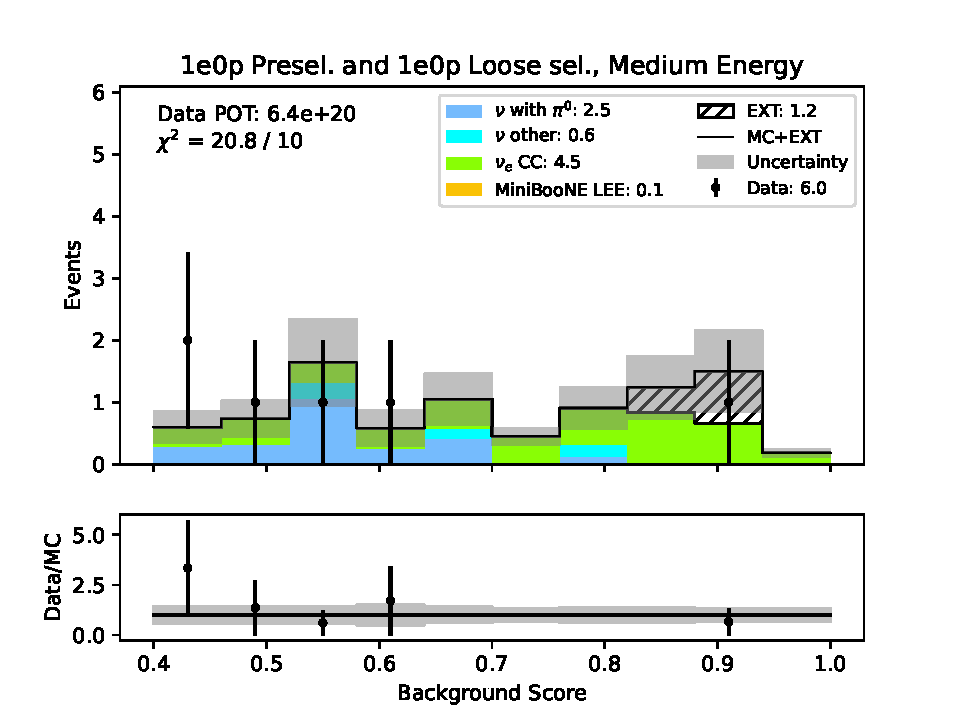
\includegraphics[width=\linewidth]{technote/Sidebands/Figures/NearSideband/near_sideband_bkg_score_run123_ZP_ZPLOOSESEL_MEDIUM_ENERGY.pdf}
        \caption{Loose selection, runs 1-3.}
    \end{subfigure}
    \begin{subfigure}{0.5\linewidth}
        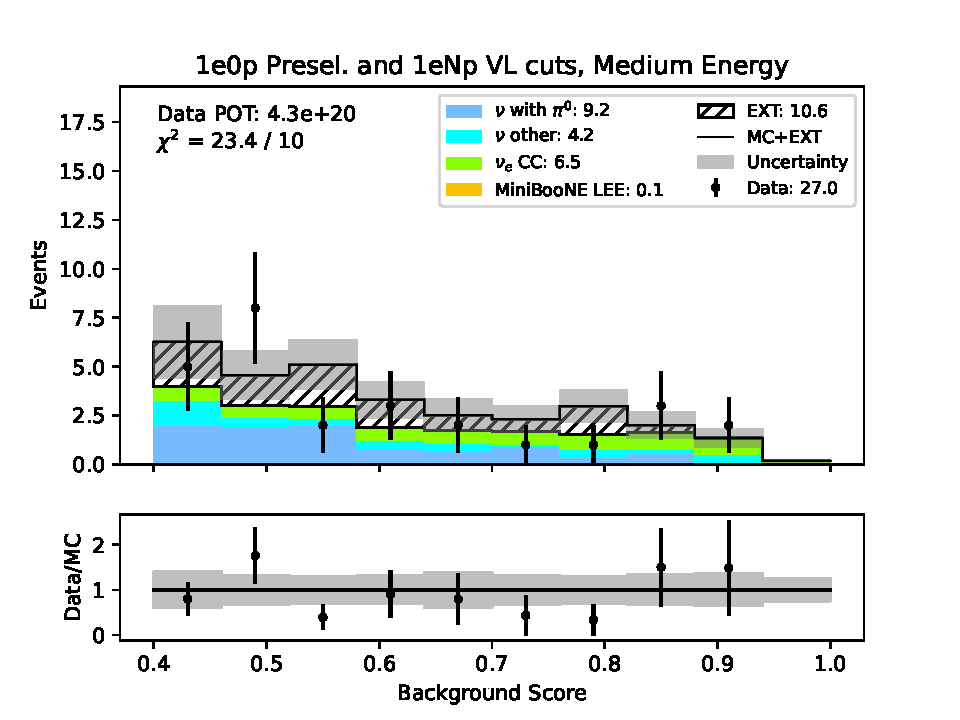
\includegraphics[width=\linewidth]{technote/Sidebands/Figures/NearSideband/near_sideband_bkg_score_run4b4c4d5_ZP_ZP_MEDIUM_ENERGY.pdf}
        \caption{$\nu_e$ preselection, runs 4-5.}
    \end{subfigure}%
    \begin{subfigure}{0.5\linewidth}
        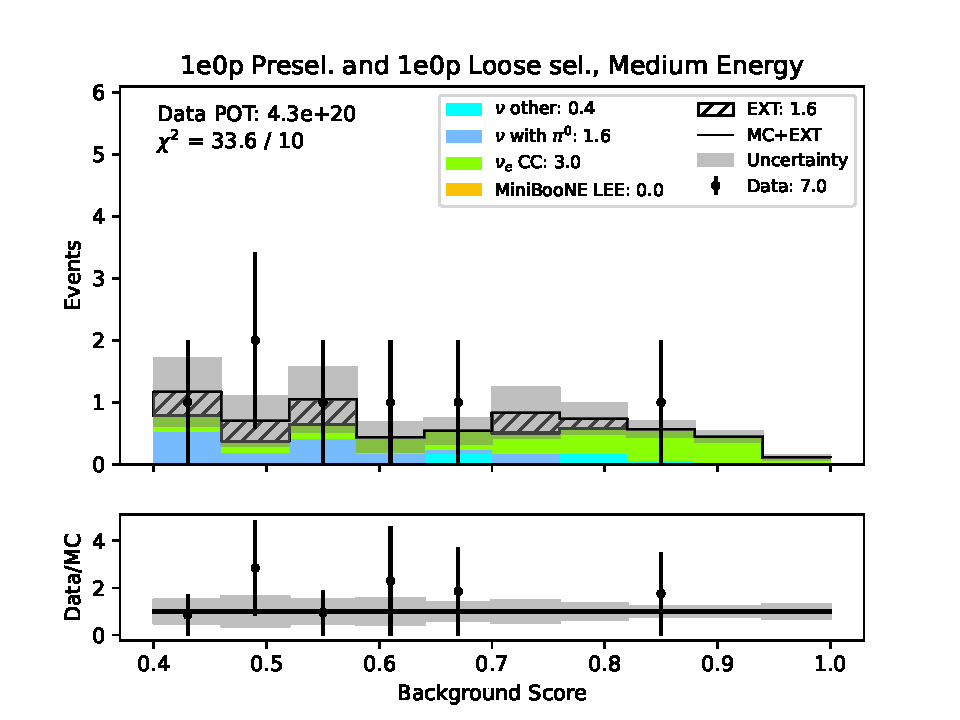
\includegraphics[width=\linewidth]{technote/Sidebands/Figures/NearSideband/near_sideband_bkg_score_run4b4c4d5_ZP_ZPLOOSESEL_MEDIUM_ENERGY.pdf}
        \caption{Loose selection, runs 4-5.}
    \end{subfigure}
    \begin{subfigure}{0.5\linewidth}
        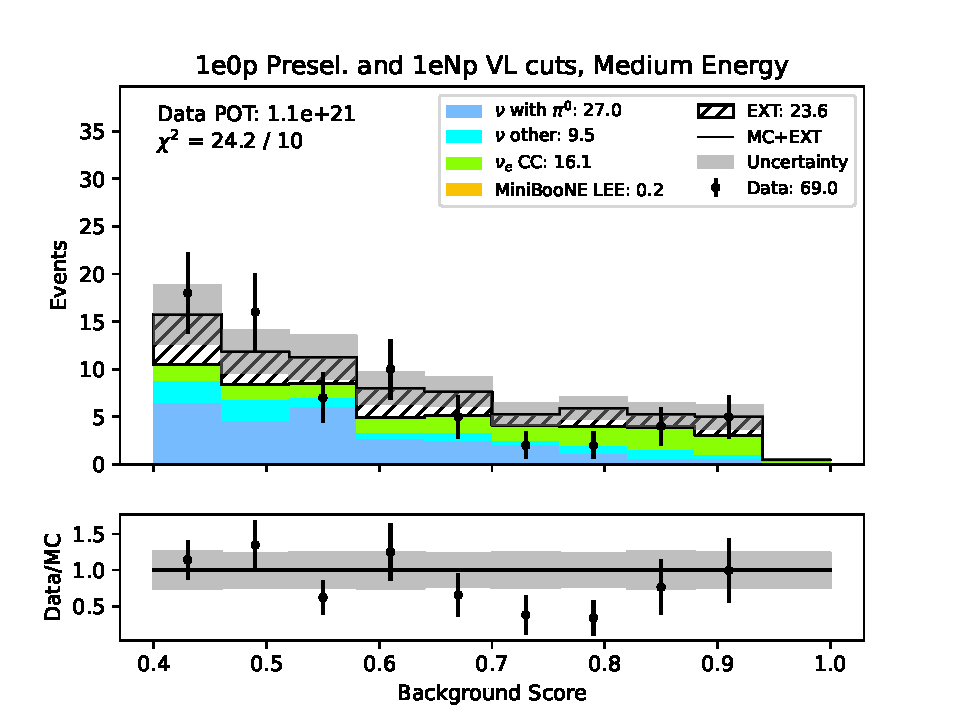
\includegraphics[width=\linewidth]{technote/Sidebands/Figures/NearSideband/near_sideband_bkg_score_run1234b4c4d5_ZP_ZP_MEDIUM_ENERGY.pdf}
        \caption{$\nu_e$ preselection, runs 1-5.}
    \end{subfigure}%
    \begin{subfigure}{0.5\linewidth}
        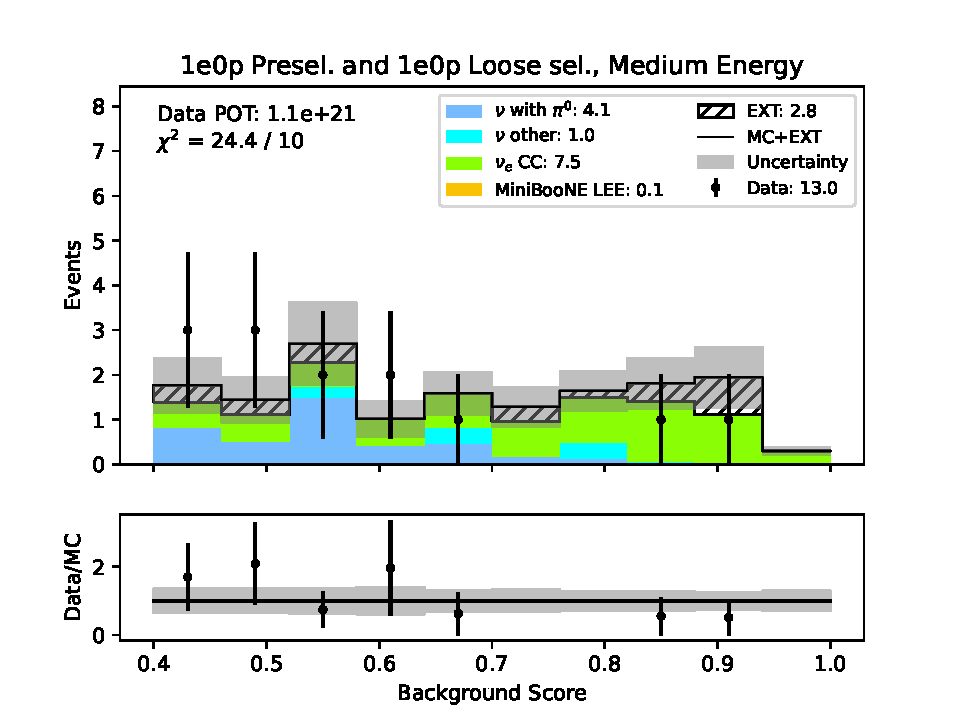
\includegraphics[width=\linewidth]{technote/Sidebands/Figures/NearSideband/near_sideband_bkg_score_run1234b4c4d5_ZP_ZPLOOSESEL_MEDIUM_ENERGY.pdf}
        \caption{Loose selection, runs 1-5.}
    \end{subfigure}
    \caption{Data and MC simulation comparisons in the 1e0p medium energy sideband.}
\end{figure}

